%% ============================================================
%%  Extended Agentic SABRE — IEEE Transactions on Information
%%  Forensics and Security (TIFS)
%%  IEEEtran journal class, two-column
%% ============================================================
\documentclass[journal]{IEEEtran}

\usepackage{amsmath,amssymb,amsfonts}
\usepackage{graphicx}
\usepackage{booktabs}
\usepackage{multirow}
\usepackage{array}
\usepackage{siunitx}
\usepackage{float}
\usepackage{algorithm}
\usepackage{algpseudocode}
\usepackage{url}
\usepackage{xcolor}
\usepackage[normalem]{ulem}
\usepackage{subcaption}
\usepackage{cite}

%% Macros
\newcommand{\phat}{\hat{p}}
\newcommand{\smax}{\sigma_{\max}}
\newcommand{\sem}{\mathrm{sem}}
\newcommand{\beh}{\mathrm{beh}}
\newcommand{\know}{\mathrm{know}}
\newcommand{\tauh}{\tau_{\mathrm{high}}}
\newcommand{\klow}{\kappa_{\mathrm{low}}}
\DeclareMathOperator{\balAcc}{bal\_acc}
\DeclareMathOperator{\escRate}{esc\_rate}

\begin{document}

\title{Extended Agentic SABRE: Multi-Modal Ransomware Detection via
Uncertainty-Driven Triage, Conformal Guarantees, and Expert-Guided
Continual Adaptation}

\author{Henry~Kabuye,
        Biju~Issac,~\IEEEmembership{Member,~IEEE,}
        Rahul~Yumlembam,
        and~Jeyamohan~Neera%
\thanks{H.~Kabuye, B.~Issac, R.~Yumlembam, and J.~Neera are with the
Department of Computer and Information Sciences, Northumbria University,
Newcastle Upon Tyne, UK.
E-mail: \{kabuyehenry2017, bissac, rahul.yumlembam, jeyamohan.neera\}@northumbria.ac.uk.}%
\thanks{B.~Issac is the corresponding author.
E-mail: bissac@ieee.org.}%
\thanks{Manuscript received April 2026.}}

\markboth{IEEE Transactions on Information Forensics and Security}%
{Kabuye \emph{et al.}: Extended Agentic SABRE}

\maketitle

%%------------------------------------------------------------
\begin{abstract}
Ransomware remains among the most operationally damaging classes of malware,
yet existing detectors typically exploit a single signal modality and provide
no principled mechanism for expressing uncertainty or handling novel attack
variants at deployment time.
We present \textbf{SABRE+} (Scalable Agent-Based Ransomware Evidence),
a multi-agent detection architecture that fuses three complementary evidence
sources: a convolutional behavioral agent operating on 16-dimensional runtime
telemetry features extracted from 10-second execution windows, a semantic agent
embedding PE static structure via a sentence transformer, and a knowledge agent
encoding ATT\&CK tactic profiles derived from threat-intelligence transcripts.
All agents employ Monte Carlo Dropout for uncertainty quantification, enabling
a three-way triage decision --- \textsc{Detect}, \textsc{Benign}, or
\textsc{Escalate} --- rather than a binary verdict.
A Mondrian conformal prediction wrapper provides formal, distribution-free
coverage guarantees on triage outcomes.

We evaluate SABRE+ on RanSMAP (35,857 windows, 15 hardware configurations,
12 families), RDset (138,047 PE samples), and RansKnow (307 ATT\&CK
transcripts) using frozen session-level splits across four generalisation axes.
Across six independent training seeds, the behavioral agent achieves
AUROC\,=\,$0.9605 \pm 0.0030$; knowledge fusion ([B+K]) raises this to
$0.9836 \pm 0.0009$.
Under realistic 5\% ransomware prevalence, [B+K] achieves AUPRC\,=\,0.898,
reducing false positives by 31\% over the behavioral baseline.
On unseen concurrent-execution traces, the system detects 83.8\% of ransomware
despite no concurrent-execution training examples.
Under worst-case feature-space mimicry, the uncertainty mechanism holds triage
coverage at 91.9\%.
At 99\% conformal coverage, [B+K] auto-classifies 77\% of traffic with 99.1\%
detection precision, escalating the remaining 23\% to analyst review.
An expert feedback loop with Elastic Weight Consolidation achieves the lowest
false-negative count (515) under OOD family drift with negligible catastrophic
forgetting ($\Delta$AUPRC\,=\,0.001 on retained families).
\end{abstract}

\begin{IEEEkeywords}
Ransomware detection, behavioral analysis, multi-agent systems, uncertainty
quantification, conformal prediction, continual learning, threat intelligence,
Monte Carlo Dropout.
\end{IEEEkeywords}


%%------------------------------------------------------------
\section{Introduction}
\label{sec:intro}

\IEEEPARstart{R}{ansomware} has emerged as the defining cyber threat of the
past decade.
By encrypting victim files and demanding payment for decryption keys,
ransomware attacks have disrupted hospitals, shut down fuel pipelines,
paralysed municipal governments, and cost organisations an estimated
\$20\,billion globally in 2021 alone --- a figure projected to exceed
\$265\,billion by 2031~\cite{cybersecurity_ventures_2022}.
Unlike traditional malware, ransomware's damage is immediate, highly visible,
and often irreversible: encrypted files cannot be recovered without either the
decryption key or a prior backup, and paying the ransom provides no guarantee
of decryption.
The operational consequences of a missed detection are therefore far more
severe than the operational friction of a false alarm.

Existing detection approaches fall into three broad categories, each with a
structural limitation that makes it insufficient on its own.
\textbf{Signature-based} detectors match file hashes or byte patterns against
a threat intelligence database; they are trivially evaded by obfuscation,
packing, and polymorphism, and provide zero-day coverage only after a family
has already been catalogued.
\textbf{Static PE analysis} --- inspecting the structure of a Portable
Executable file before execution --- can capture section entropy, import
tables, and structural anomalies indicative of packed code.
Machine-learning classifiers trained on static features achieve high accuracy
on known families~\cite{rdset_2021}, but remain inherently offline: static
analysis cannot observe the file-encryption loop, the ransom note drop, or the
shadow-copy deletion that together constitute ransomware behaviour.
\textbf{Dynamic/behavioural} analysis addresses this by monitoring execution
at runtime (system calls, I/O patterns, memory access) and detecting the
characteristic signatures of file encryption in motion.
Behavioural detectors are harder to evade without also losing the attack's
effectiveness, but they operate without context: they know \emph{what} a
process is doing but not \emph{who} is doing it or \emph{why}, making
family-level intelligence impossible from telemetry alone.

No production-grade system currently integrates all three evidence streams
under a unified uncertainty-aware decision framework.
More critically, no existing approach formalises the question of \emph{when
to trust the detector's verdict}.
In any realistic deployment, the class distribution is severely skewed ---
ransomware constitutes a small minority of execution events --- and the
consequences of a missed detection are asymmetric.
An optimal system should distinguish between high-confidence detections
(auto-flag), high-confidence benign events (auto-clear), and ambiguous cases
requiring analyst review (escalate).
Without a principled mechanism for this three-way triage, either false-positive
rates overwhelm analyst queues, or high-uncertainty true positives are silently
missed.

We present \textbf{SABRE+} (Scalable Agent-Based Ransomware Evidence),
a multi-agent architecture that addresses these gaps.
SABRE+ coordinates three specialist agents --- a \textbf{Behavioral agent}
operating on runtime I/O and memory telemetry, a \textbf{Semantic agent}
classifying PE file structure via a sentence-transformer embedding, and a
\textbf{Knowledge agent} encoding ATT\&CK tactic profiles from
threat-intelligence transcripts --- under a shared Monte Carlo Dropout
uncertainty framework.
Each agent contributes a probability estimate and an epistemic uncertainty;
the fused uncertainty drives a three-way triage decision.
A Mondrian conformal prediction wrapper converts the fused scores into
prediction sets with guaranteed marginal coverage, so that auto-flagged
samples carry a formal bound on detection precision.
An expert feedback loop with Elastic Weight Consolidation (EWC) allows the
behavioral agent to adapt to novel families at deployment time without
catastrophic forgetting of established detection patterns.

We evaluate SABRE+ on three complementary public datasets spanning runtime
telemetry (RanSMAP: 35,857 windows across 15 hardware configurations and 12
malware families), static PE structure (RDset: 138,047 PE files), and threat
intelligence (RansKnow: 307 ATT\&CK-annotated transcripts).
Experiments use frozen session-level splits across four generalisation axes
(random stratification, family holdout, hardware holdout, and temporal
holdout), replicated across six independent training seeds to quantify
reproducibility.

\textbf{The main contributions of this paper are:}

\begin{enumerate}

\item \textbf{Multi-modal multi-agent architecture.}
We introduce the first ransomware detection system to unify runtime
behavioural telemetry, PE static semantics, and ATT\&CK knowledge features in
a single inference pipeline, with mean fusion controllable by agent
availability at deployment time.

\item \textbf{Uncertainty-driven triage.}
MC-Dropout uncertainty quantification enables a \textsc{Detect} /
\textsc{Benign} / \textsc{Escalate} triage that, under worst-case
feature-space mimicry attacks, maintains \textbf{91.9\% triage coverage}
while the direct detection rate falls to 81.7\% --- recovering 10.2\,pp
through analyst escalation of high-uncertainty samples.

\item \textbf{Conformal triage with formal coverage guarantees.}
Mondrian conformal prediction applied to temperature-scaled fused scores
achieves empirical coverage within 1.2\,pp of the target at all tested levels.
At 99\% coverage, [B+K] auto-classifies 77\% of traffic with
\textbf{99.1\% detection precision}, escalating 23\% for analyst review.

\item \textbf{Continual learning under distribution shift.}
An EWC-regularised expert feedback loop reduces false negatives under OOD
family arrival (515 vs.\ 520 for no-update) with negligible catastrophic
forgetting (probe AUPRC drop\,=\,0.001), identifying the labelling budget ---
not the update strategy --- as the primary constraint on adaptation speed.

\item \textbf{Comprehensive generalisation evaluation.}
Across six seeds, the behavioral agent achieves
AUROC\,=\,$0.9605 \pm 0.0030$ on the canonical split,
$0.9387 \pm 0.0058$ on unseen hardware, and $0.9603 \pm 0.0054$ under
temporal holdout.
Family-level generalisation degrades to $0.7069 \pm 0.0104$ for wholly unseen
ransomware lineages, quantifying a clear research frontier.

\item \textbf{Concurrent-execution robustness.}
On the RanSMAP mix partition --- simultaneous benign and ransomware execution
on unseen hardware --- [B] detects \textbf{83.8\%} of ransomware windows with
no concurrent-execution training examples.
SDelete co-execution reduces detection to 27.1\% (\texttt{SDelete\_REvil}),
with MC-Dropout uncertainty correctly routing the remaining ambiguous windows
to escalation.

\item \textbf{Deployment-grade efficiency.}
The [B+K] pipeline runs at \textbf{4.969\,ms} median end-to-end latency
(p95\,=\,5.997\,ms) on a single GPU --- consuming 0.05\% of a 10-second
telemetry window --- and supports over 2,000 concurrent monitored streams.
The behavioral agent weighs 8,385 parameters (32.8\,KB), making it suitable
for endpoint or embedded deployment without a GPU.

\end{enumerate}

The remainder of this paper is organised as follows.
Section~\ref{sec:related} surveys related work.
Section~\ref{sec:preliminaries} states the threat model and mathematical
preliminaries.
Section~\ref{sec:architecture} describes the SABRE+ system architecture,
including the three agent designs and the fusion and triage modules.
Section~\ref{sec:experiments} presents the experimental datasets and
evaluation protocol.
Section~\ref{sec:triage_cl} describes the triage and continual learning
mechanisms in detail.
Section~\ref{sec:results} reports experimental results across all evaluation
dimensions.
Section~\ref{sec:limitations} discusses limitations and directions for future
work, and Section~\ref{sec:conclusion} concludes.

%%------------------------------------------------------------
\section{Related Work}
\label{sec:related}

\subsection{Ransomware Detection}
Early detection systems relied on static signatures and
API call sequences~\cite{fernando2020study}.
The transition to deep learning brought CNN and LSTM architectures
operating on system-call traces, filesystem activity, and network
flows~\cite{zahoora2022Deep,alraizza2023ransomware}, achieving strong
in-distribution performance but failing under distributional shift.
Survey work~\cite{razaulla2023age} identifies concept drift as the
primary operational challenge for deployed detectors.
FeSAD~\cite{Fernando2024FeSAD} addresses drift with a feature-selection
framework but lacks uncertainty-aware decision logic.
LLM-LADE~\cite{ZhangLZYHY25} leverages large language models for
log-based anomaly detection with partial symbolic reasoning, but
does not quantify uncertainty or produce triage decisions.

\subsection{Uncertainty Quantification in Security}
Bayesian deep learning has been applied to network intrusion
detection~\cite{Doan2024uncertainBay}, malware
classification~\cite{kabuye2025explainable}, and vulnerability
assessment.
MC Dropout~\cite{gal2016dropout} is the most practical approach for
production systems, approximating Bayesian inference with a single
trained model at the cost of $T$ forward passes per sample.
Temperature scaling~\cite{guo2017calibration} corrects the
overconfidence of trained neural classifiers and is used here as a
post-hoc calibration step.
The critical missing link in prior work is the
\emph{operational use} of uncertainty: existing systems report it but
do not use it to govern agent behaviour or inter-agent communication.

\subsection{Knowledge-Augmented Detection}
Neuro-symbolic methods integrate structured knowledge with
statistical models to improve generalisation under distributional
shift~\cite{Ispahany2024Survey}.
In the ransomware domain, ATT\&CK-aligned feature engineering has
been used for rule-based pre-filtering~\cite{razaulla2023age}, but has
not been coupled with learned uncertainty estimation.
The RansKnow dataset introduced here is the first knowledge resource
for ransomware detection derived from structured analysis of practitioner
video transcripts.

\subsection{Multi-Agent Security Frameworks}
Multi-agent approaches to intrusion detection decompose detection
into specialised sub-agents whose outputs are
combined~\cite{MultiAgentAdaptiveDetection2023}.
Soltani et al.~\cite{MultiAgentAdaptiveDetection2023} propose an
adaptive multi-agent intrusion detection system but do not equip
agents with uncertainty estimates or inter-agent communication.
The two-agent SABRE baseline~\cite{kabuye2025sabre_eswa} demonstrated
the benefit of modality-specific agents with uncertainty-aware fusion,
but agents remain isolated.
SABRE+ adds a third modality and a formal peer consultation protocol.

\subsection{Continual Learning in Threat Detection}
Concept drift under evolving adversarial strategies requires detectors
to adapt without retraining from scratch~\cite{Ceschin2022ConceptDrift}.
Experience replay~\cite{rolnick2019experience} and elastic weight
consolidation prevent catastrophic forgetting during incremental updates.
SABRE+'s Expert Feedback Loop combines both techniques to incrementally adapt
the behavioral agent's classifier head while leaving the convolutional feature
backbone frozen, limiting the risk of catastrophic forgetting to a small
parameter subset.

%%------------------------------------------------------------
\section{Threat Model and Preliminaries}
\label{sec:preliminaries}

\subsection{Threat Model}
We consider a defender operating an enterprise endpoint detection and
response (EDR) pipeline against an adversary deploying ransomware with
the following capabilities:
(i) binary polymorphism and metamorphism to evade signature matching;
(ii) living-off-the-land (LotL) techniques to blend runtime telemetry
with benign system activity;
(iii) gradual deployment (slow encryption, staged loaders) to defeat
burst-based behavioural detectors;
(iv) access to the defender's detection policy \emph{only} through
repeated probing, not to model weights or training data.
We do \emph{not} assume the adversary can suppress ATT\&CK-aligned tool
usage (Cobalt Strike for lateral movement, Rclone for exfiltration,
etc.) because these tools serve operational purposes the adversary
cannot easily replace.
We do not claim to prevent zero-day exploits or fully novel
attack chains absent from the training distribution.

\subsection{Monte Carlo Dropout Inference}
Given a neural network $f_\theta$ with Dropout layers, MC Dropout
approximates the posterior predictive distribution by performing $T$
stochastic forward passes at inference time.
For a feature vector $\mathbf{x}$:
\begin{align}
\bar{p} &= \frac{1}{T}\sum_{t=1}^{T} f_{\theta}^{(t)}(\mathbf{x}),
\label{eq:mc_mean}\\
\sigma  &= \sqrt{\frac{1}{T}\sum_{t=1}^{T}\left(f_{\theta}^{(t)}(\mathbf{x})
           - \bar{p}\right)^2}.
\label{eq:mc_std}
\end{align}
Here $\bar{p}\in[0,1]$ is the predictive mean probability and
$\sigma\in[0,\infty)$ is the empirical standard deviation across passes,
serving as a proxy for epistemic uncertainty.

\subsection{Score Vector}
Each agent $i\in\{\sem,\beh,\know\}$ produces a tuple
$(\bar{p}_i, \sigma_i)$.
After peer consultation the six-dimensional score vector is:
\begin{equation}
\mathbf{v} =
\begin{bmatrix}
\bar{p}_\sem^* \\ \bar{p}_\beh^* \\ \bar{p}_\know^* \\
\sigma_\sem   \\ \sigma_\beh   \\ \sigma_\know
\end{bmatrix}
\in \mathbb{R}^6,
\label{eq:scorevec}
\end{equation}
where $\bar{p}_i^*$ denotes the post-consultation probability
(equal to $\bar{p}_i$ when consultation did not fire for agent $i$)
and all $\sigma_i$ are the original MC Dropout standard deviations.


%%------------------------------------------------------------
\section{Extended Agentic SABRE Architecture}
\label{sec:architecture}

\subsection{System Overview}

\begin{figure*}[t]
  \centering
  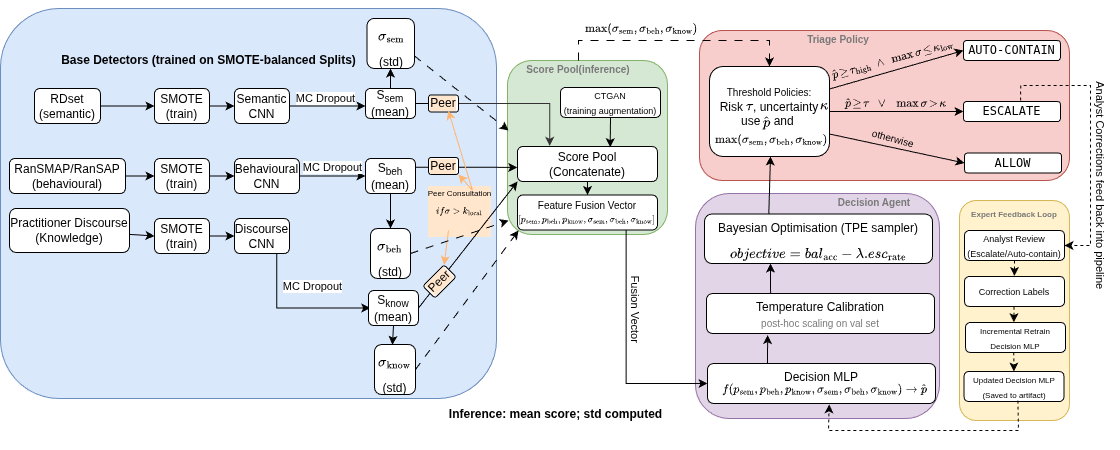
\includegraphics[width=\linewidth]{Figures/Prop_Agentic_Sabre_27_04_2026_3Agents_Fullpipeline.png}
  \caption{Extended Agentic SABRE+ pipeline. Three specialist agents
  (Behavioral CNN, Semantic CNN, Knowledge CNN) produce
  predictive mean--uncertainty pairs $(\bar{p}_i, \sigma_i)$ via MC-Dropout.
  The Fusion Layer averages active agents into a fused probability
  $\bar{p}_{\mathrm{fused}}$ and fused uncertainty $\sigma_{\mathrm{fused}}$.
  The Triage Decision Module maps the fused pair to
  \texttt{DETECT}, \texttt{ESCALATE}, or \texttt{BENIGN}.
  A Mondrian Conformal Wrapper converts temperature-scaled probabilities
  into prediction sets with formal, distribution-free coverage guarantees.
  \texttt{ESCALATE} decisions queue for analyst review; verified labels
  feed the EWC-regularised Expert Feedback Loop, which incrementally
  retrains the Behavioral agent to adapt to novel ransomware families.}
  \label{fig:pipeline}
\end{figure*}

Fig.~\ref{fig:pipeline} illustrates the complete pipeline.
The system coordinates three specialist agents, each operating on a distinct
modality: runtime I/O and memory telemetry (Behavioral), static PE-header
semantics (Semantic), and ATT\&CK threat-intelligence discourse (Knowledge).
Agents are trained independently on their native datasets and frozen.
At inference, each active agent performs $T=10$ MC-Dropout forward passes,
producing a predictive mean $\bar{p}_i$ and epistemic uncertainty $\sigma_i$.
The Fusion Layer averages active agents into a fused probability and fused
uncertainty, which the Triage Decision Module maps to \texttt{DETECT},
\texttt{ESCALATE}, or \texttt{BENIGN}.
A Mondrian Conformal Wrapper converts temperature-scaled probabilities into
prediction sets with formal coverage guarantees.
\texttt{ESCALATE} decisions are queued for analyst review; verified labels
are routed to the Expert Feedback Loop for incremental adaptation.

\subsection{Semantic Agent}

The Semantic Agent operates on 384-dimensional PE-header embeddings
derived from the RDset dataset~\cite{kabuye2025explainable}.
Embeddings are computed from structured metadata (import tables, section
entropy, PE flags, version strings) and capture the static representational
fingerprint of each executable.
The agent architecture is a five-layer CNN over the embedding vector
with ReLU activations, batch normalisation, and a Dropout layer
($p_{\mathrm{drop}}=0.3$) before the final sigmoid unit.
At inference, $T=10$ MC Dropout passes yield $(\bar{p}_\sem, \sigma_\sem)$.
From the trained scaler statistics, $\bar{\sigma}_\sem \approx 2.75
\times 10^{-8}$, confirming near-deterministic confidence on the
RDset distribution---a consequence of the well-separated class-conditional
embedding clusters documented in~\cite{kabuye2025sabre_eswa}.

\subsection{Behavioural Agent}

The Behavioural Agent operates on 16-dimensional runtime telemetry
features extracted from the RanSMAP dataset~\cite{kabuye2025sabre_eswa},
capturing LBA/GPA variance, memory operation counts, and I/O entropy
statistics.
The architecture mirrors the Semantic CNN with a 1D-CNN backbone and
MC Dropout.
The trained scaler indicates $\bar{\sigma}_\beh \approx 0.0138$
($\mathrm{std}\approx 0.0258$), reflecting the greater behavioural
overlap between benign and ransomware-infected hosts compared to the
static embedding space.
On balanced held-out evaluation (1000 samples per class) the agent
achieves accuracy 0.9945 and AUC 0.9967; the imbalanced evaluation
on the full RanSMAP class distribution (598:1 malicious:benign ratio)
yields AUC~0.6030~\cite{kabuye2025sabre_eswa}, confirming that rank-based
separation is substantially harder under extreme class imbalance.

\subsection{Knowledge Agent and RansKnow Dataset}
\label{subsec:knowledge_agent}

\subsubsection{RansKnow Dataset}
RansKnow is a novel dataset of 307~samples (140 ransomware-relevant,
167 benign) derived from structured analysis of YouTube security
practitioner content, including threat-intelligence briefings, DFIR
(digital forensics and incident response) walkthroughs, and
ransomware family deep-dives published by analyst channels.
Each sample corresponds to one video and is represented by
23~structured features (Table~\ref{tab:ransknow_features}):
10~MITRE ATT\&CK tactic frequency counts, 8~ransomware-ecosystem
tool mention counts, 3~platform signal indicators, and 2~aggregate
mention totals.
Labels are derived heuristically:
a sample is \emph{ransomware-relevant} if
$\texttt{Tactic\_Total\_Mentions} > 10$ or
$\texttt{Tool\_Total\_Mentions} > 2$,
reflecting the empirical observation that legitimate ransomware
analyses consistently reference both high-tactic-frequency deployment
chains and specific attacker tooling.

\begin{table}[t]
\centering
\caption{RansKnow dataset feature groups.}
\label{tab:ransknow_features}
\begin{tabular}{lll}
\toprule
\textbf{Group} & \textbf{Count} & \textbf{Examples} \\
\midrule
ATT\&CK tactic counts & 10 &
  Initial Access, Exfiltration, Impact \\
Tool mention counts   & 8  &
  Cobalt Strike, Rclone, Mimikatz \\
Platform signals      & 3  &
  Windows, Linux, ESXi \\
Aggregate totals      & 2  &
  Tactic\_Total, Tool\_Total \\
\midrule
\textbf{Total} & \textbf{23} & 307 samples \\
\bottomrule
\end{tabular}
\end{table}

\subsubsection{Architecture}
The Knowledge CNN operates on the 23-dimensional feature vector.
The architecture consists of a 1D convolution layer
(16 filters, kernel size 3, same padding), ReLU activation,
max-pooling (stride 2), Dropout ($p_{\mathrm{drop}}=0.3$), a
flatten layer, and two fully connected layers
(64 hidden units, sigmoid output).
MC Dropout is applied adaptively: passes continue from a minimum of
$T_{\min}=5$ until the running standard deviation of
$\sigma_{\know}$ converges within tolerance $\delta=10^{-3}$,
capped at $T_{\max}=50$.
Trained scaler statistics indicate
$\bar{\sigma}_{\know} \approx 0.0499$ ($\mathrm{std}\approx 0.0734$),
reflecting higher epistemic uncertainty than the Semantic Agent but
comparable to the Behavioural Agent---consistent with the modest
dataset size.

\subsubsection{Complementarity}
The three agents cover distinct attack surfaces.
The Semantic Agent is strong on known-family PE variants but blind to
novel polymorphic samples with unfamiliar byte patterns.
The Behavioural Agent captures runtime encryption dynamics but may be
confused by LotL techniques that generate benign-looking telemetry.
The Knowledge Agent is strong precisely when practitioners have
documented a deployment chain---i.e., for well-known campaigns with
ATT\&CK-mapped tooling---irrespective of PE structure or runtime
behaviour.
Together, the three agents provide overlapping but non-identical
coverage of the ransomware detection surface.

\subsection{Fusion Layer}
\label{subsec:fusion}

Let $\mathcal{A} \subseteq \{\sem, \beh, \know\}$ denote the set of active agents for a
given sample.
The Fusion Layer computes an unweighted mean over all active agents:
\begin{align}
\bar{p}_{\mathrm{fused}} &= \frac{1}{|\mathcal{A}|} \sum_{i \in \mathcal{A}} \bar{p}_i,
\label{eq:fused_prob}\\
\sigma_{\mathrm{fused}} &= \frac{1}{|\mathcal{A}|} \sum_{i \in \mathcal{A}} \sigma_i.
\label{eq:fused_unc}
\end{align}
Mean fusion is availability-aware by construction: absent agents are simply omitted from
$\mathcal{A}$ without requiring model retraining.
The primary limitation of mean fusion is structural miscalibration when agents have
heterogeneous probability scales; the Mondrian conformal wrapper (below) provides
post-hoc coverage guarantees that are valid regardless of calibration quality.

\subsection{Triage Decision Module}
\label{subsec:triage}

After temperature scaling (Section~\ref{sec:triage_cl}), the calibrated fused probability
$\tilde{p}_{\mathrm{fused}}$ and fused uncertainty $\sigma_{\mathrm{fused}}$ are mapped
to one of three outcomes:
\begin{equation}
\text{outcome}(\mathbf{x}) = \begin{cases}
  \texttt{DETECT}   & \text{if } \tilde{p}_{\mathrm{fused}} \geq 0.5, \\
  \texttt{ESCALATE} & \text{if } \tilde{p}_{\mathrm{fused}} < 0.5 \;\text{and}\;
                      \sigma_{\mathrm{fused}} \geq \tau, \\
  \texttt{BENIGN}   & \text{otherwise.}
\end{cases}
\label{eq:triage}
\end{equation}
The \texttt{ESCALATE} branch captures samples the model considers probably benign but is
uncertain about; these are routed to analyst review rather than silently auto-cleared.
The uncertainty threshold $\tau = 0.10$ is the 90th percentile of $\sigma_{\mathrm{fused}}$
over benign validation samples, bounding the false-\texttt{ESCALATE} rate to at most 10\%
on in-distribution clean traffic.
\emph{Triage coverage} (TC) denotes the fraction of true ransomware samples that receive
either \texttt{DETECT} or \texttt{ESCALATE}; it is the primary robustness criterion under
adversarial feature manipulation (Section~\ref{sec:results}).

\subsection{Conformal Prediction Wrapper}
\label{subsec:conformal_arch}

A post-hoc Mondrian inductive conformal prediction (ICP) layer converts
temperature-scaled fused probabilities into \emph{prediction sets} with formal,
distribution-free coverage guarantees~\cite{vovk_conformal_2005}.
Class-conditional nonconformity thresholds $q_0, q_1$ are fitted on the validation split
at significance level $\varepsilon$; the prediction set $C(\mathbf{x})$ satisfies:
\begin{equation}
\Pr\!\bigl[y \in C(\mathbf{x}) \mid y = c\bigr] \geq 1-\varepsilon, \quad c \in \{0,1\}.
\label{eq:coverage_arch}
\end{equation}
Prediction sets map to triage outcomes as:
$C\!=\!\{1\}\!\Rightarrow\!\texttt{DETECT}$;
$C\!=\!\{0\}\!\Rightarrow\!\texttt{BENIGN}$;
$C\!=\!\{0,1\}\!\Rightarrow\!\texttt{ESCALATE}$;
$C\!=\!\emptyset\!\Rightarrow\!\texttt{DETECT}$ (conservative edge).
The full Mondrian formulation and empirical validation are given in
Section~\ref{sec:triage_cl}.

\subsection{Availability-Aware Operation}
\label{subsec:availability}

Table~\ref{tab:deployment_configs} summarises the four supported deployment configurations.
The {[}B{]} configuration passes the Behavioral agent's output directly to triage, with
conformal thresholds recomputed on {[}B{]}-only scores.
In {[}B{+}K{]}, the Knowledge agent contributes its family-matched ATT\&CK prior; for
families absent from RansKnow the corpus-mean vector provides a near-uniform prior and
the system logs a coverage-gap warning.
The Semantic agent ({[}S{]}) is excluded from the primary evaluation pipeline because it
requires an unobfuscated PE file unavailable during live execution of packed ransomware;
its AUROC = 1.000 on RDset reflects closed-set structural separability
(Section~\ref{sec:results}).

\begin{table}[t]
\centering
\caption{SABRE+ deployment configurations under partial agent availability.}
\label{tab:deployment_configs}
\setlength{\tabcolsep}{3pt}
\begin{tabular}{lp{2.1cm}p{2.3cm}}
\toprule
\textbf{Config.} & \textbf{Input requirements} & \textbf{Typical scenario} \\
\midrule
{[}B{]}       & Runtime telemetry    & Packed binaries; PE unavailable \\
{[}S{]}       & PE file only         & Offline pre-execution scan \\
{[}K{]}       & Family name resolved & Threat-intel triage \\
{[}B{+}K{]}   & Telemetry + family   & Standard EDR deployment \\
{[}B{+}S{+}K{]} & All three inputs   & Sandboxed deep analysis \\
\bottomrule
\end{tabular}
\end{table}

%%------------------------------------------------------------
\section{Triage and Continual Learning}
\label{sec:triage_cl}

This section provides the mathematical formulations underlying SABRE+'s inference
pipeline and online adaptation mechanism.
Section~\ref{sec:architecture} introduced these components architecturally;
here we give the specifications used in the experimental evaluation
(Section~\ref{sec:results}).

\subsection{MC-Dropout Uncertainty Estimation}

At inference, each agent runs in MC-Dropout mode: evaluation mode except for Dropout
layers, which remain active via selective module traversal.
For $T$ stochastic passes on input $\mathbf{x}$, agent $i$ produces:
\begin{equation}
\bar{p}_i = \frac{1}{T}\sum_{t=1}^{T} p_i^{(t)},
\qquad
\sigma_i = \sqrt{\frac{1}{T}\sum_{t=1}^{T}\bigl(p_i^{(t)} - \bar{p}_i\bigr)^2}.
\label{eq:mc_dropout}
\end{equation}
Under the MC-Dropout variational approximation~\cite{gal2016dropout},
$\bar{p}_i$ estimates the posterior predictive mean and $\sigma_i$
estimates posterior predictive standard deviation.
High $\sigma_i$ arises when dropout mask configurations disagree: the sample is near
a decision boundary, out-of-distribution, or presents an underrepresented feature pattern.

All reported results use $T=10$ passes.
Validation-set profiling confirms that $95\%$ of samples have running
$\mathrm{std}(\{p^{(t)}\})$ within $10^{-3}$ of their $T=50$ value by $T=8$.
The $T=10$ latency overhead is $3.70\times$ a deterministic pass
(Section~\ref{sec:results}).

\subsection{Fusion and Uncertainty Aggregation}

Fused probability and fused uncertainty are defined in
Eqs.~\eqref{eq:fused_prob}--\eqref{eq:fused_unc}.
Mean fusion over uncertainties is conservative: one high-$\sigma$ agent and one
low-$\sigma$ agent yield an intermediate fused uncertainty, reflecting the average
epistemic state.
Under adversarial feature-space mimicry (Section~\ref{sec:results}), this conservatism
is beneficial: a deceived agent exhibits elevated $\sigma$ even when $\bar{p}$ falls
below the detection threshold, propagating the uncertainty signal to the triage layer.

\subsection{Uncertainty-Driven Three-Way Triage}

The triage rule (Eq.~\eqref{eq:triage}) is asymmetric by design
(Fig.~\ref{fig:triage_scatter}).
\texttt{DETECT} fires whenever $\tilde{p}_{\mathrm{fused}} \geq 0.5$ regardless of
uncertainty, accepting the risk of high-uncertainty detections (which may be false
positives) rather than silently missing high-confidence ransomware.
The \texttt{ESCALATE} branch applies only in the $\tilde{p} < 0.5$ region: a sample
the model considers probably benign but is uncertain about.
This asymmetry reflects the asymmetric cost of ransomware detection: false negatives
have irreversible operational consequences; false positives (analyst reviews) are
recoverable.

\textbf{Triage coverage.}
The primary adversarial robustness metric is:
\begin{equation}
\mathrm{TC} = \frac{|\{x \in \mathcal{R} : \text{outcome}(x) \in
    \{\texttt{DETECT},\texttt{ESCALATE}\}\}|}{|\mathcal{R}|},
\label{eq:tc}
\end{equation}
where $\mathcal{R}$ is the set of true ransomware samples.
Under worst-case feature-space mimicry, TC holds at 91.9\% while
the detection rate falls to 81.7\%, recovering 10.2~pp through escalation
(Section~\ref{sec:results}, Fig.~\ref{fig:adversarial}).

\begin{figure}[!t]
  \centering
  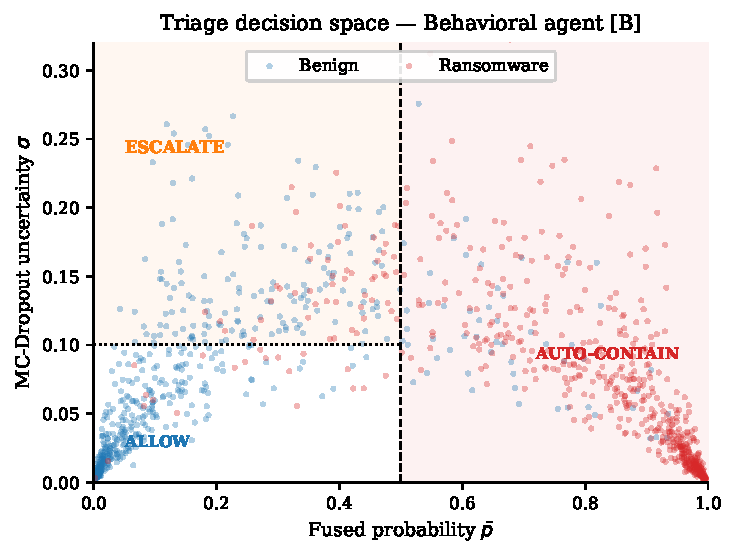
\includegraphics[width=\linewidth]{Figures/fig4_triage_scatter.pdf}
  \caption{Triage decision space for the Behavioral agent [B] on the
  random-stratified test split.
  Each point is a 10-second window coloured by true label (blue = benign,
  red = ransomware).
  The vertical dashed line at $\bar{p}=0.5$ separates \textsc{Detect} from
  the uncertain region; the horizontal dotted line at $\sigma=\tau=0.10$
  separates \textsc{Escalate} from \textsc{Benign}.}
  \label{fig:triage_scatter}
\end{figure}

\subsection{Temperature Scaling}

Raw MC-Dropout probabilities are corrected by temperature scaling~\cite{guo2017calibration}:
\begin{equation}
\tilde{p} = \sigma\!\left(\frac{\mathrm{logit}(\bar{p}_{\mathrm{fused}})}{T_{\mathrm{cal}}}\right),
\label{eq:temperature_scaling}
\end{equation}
where $T_{\mathrm{cal}} < 1$ sharpens underconfident predictions and $T_{\mathrm{cal}} > 1$
softens overconfident ones.
$T_{\mathrm{cal}}^*$ minimises NLL over the validation split:
\begin{equation}
T_{\mathrm{cal}}^* = \arg\min_{T>0}
    -\frac{1}{n_{\mathrm{val}}}\sum_{j=1}^{n_{\mathrm{val}}}
    \bigl[y_j\log\tilde{p}_j + (1{-}y_j)\log(1{-}\tilde{p}_j)\bigr].
\label{eq:temp_nll}
\end{equation}
For {[}B{]}, $T_{\mathrm{cal}} = 0.703$ reduces test ECE from $0.042$ to $0.018$.
For {[}B{+}K{]}, structural miscalibration from heterogeneous agent probability scales
limits the reduction from $0.143$ to $0.131$; this is a known limitation of mean fusion
(Section~\ref{sec:limitations}).

\subsection{Mondrian Inductive Conformal Prediction}
\label{subsec:mondrian}

The Mondrian ICP wrapper converts temperature-scaled probabilities into
\emph{prediction sets} with class-conditional, distribution-free coverage
guarantees~\cite{vovk_mondrian_2003,vovk_conformal_2005}.
For each class $c \in \{0,1\}$, the nonconformity score measures the mismatch
between the calibrated probability and label $c$:
\begin{equation}
s(\mathbf{x}, c) = \begin{cases}
  1 - \tilde{p}(\mathbf{x}) & c = 1, \\
  \tilde{p}(\mathbf{x})     & c = 0.
\end{cases}
\label{eq:nonconformity}
\end{equation}
The class-conditional threshold is the upper $(1-\varepsilon)$ quantile of calibration-set
nonconformity scores for class $c$:
\begin{equation}
q_c = \mathrm{Quantile}_{(1-\varepsilon)}\!\bigl(
    \{s(\mathbf{x}_j, c) : y_j = c,\, j \in \mathcal{D}_{\mathrm{cal}}\}\bigr),
\label{eq:mondrian_quantile}
\end{equation}
with the finite-sample adjustment $\lceil(n_c+1)(1-\varepsilon)\rceil/n_c$.
The prediction set is $C(\mathbf{x}) = \{c : s(\mathbf{x},c) \leq q_c\}$,
mapping to triage outcomes per Eq.~\eqref{eq:coverage_arch}.

\textbf{Coverage guarantee.}
Under exchangeability of calibration and test samples:
\begin{equation}
\Pr\!\bigl[y \in C(\mathbf{x}) \mid y = c\bigr] \geq 1-\varepsilon,\quad c \in \{0,1\}.
\label{eq:coverage_formal}
\end{equation}
This guarantee is \emph{distribution-free} and label-conditional (not marginal), making it
valid under class imbalance where marginal coverage would be dominated by the majority class.
Empirical validation in Section~\ref{sec:results} confirms the guarantee holds to within
1.2~pp across $\varepsilon \in \{0.10, 0.05, 0.01\}$.

\subsection{Expert Feedback Loop}
\label{subsec:efl}

The Expert Feedback Loop enables the Behavioral agent to adapt to novel ransomware families
observed at deployment time.
Only the Behavioral agent is updated; the Semantic and Knowledge agents are frozen
because their parameters depend on fixed external corpora that do not drift on the
timescale of a deployment episode.

\textbf{Stream structure.}
Experiments use the temporal holdout split in two phases:
\begin{itemize}
\item \emph{Phase~1 (steps~1--27):} Temporal validation windows (Jun~2023--Feb~2024;
  5,494~windows). No updates; establishes pre-drift AUPRC $= 0.9838$ baseline.
\item \emph{Phase~2 (steps~28--34):} Temporal test windows merged with 1,397 OOD Conti
  sub-variants (\texttt{Conti\_01}--\texttt{Conti\_07}).
  Updates enabled; 50 of each step's 200~windows labelled by the analyst (25\% budget).
\end{itemize}

\subsection{Elastic Weight Consolidation}
\label{subsec:ewc}

EWC~\cite{kirkpatrick_ewc_2017} prevents catastrophic forgetting by penalising parameter
changes proportional to their importance to previously learned detection patterns:
\begin{equation}
\mathcal{L}_{\mathrm{EWC}}(\boldsymbol{\theta}) =
\mathcal{L}_{\mathrm{CE}}(\boldsymbol{\theta})
+ \frac{\lambda}{2}\sum_i \hat{F}_i \left(\theta_i - \theta_i^*\right)^2,
\label{eq:ewc}
\end{equation}
where $\boldsymbol{\theta}^*$ are the pre-update parameters and
$\hat{F}_i$ is the $i$-th diagonal of the Fisher information matrix:
\begin{equation}
\hat{F}_i = \frac{1}{N}\sum_{n=1}^{N}
    \left(\frac{\partial}{\partial\theta_i}
    \mathcal{L}_{\mathrm{CE}}^{(n)}(\boldsymbol{\theta}^*)\right)^{\!2},
\label{eq:fisher}
\end{equation}
estimated on $N=300$ training windows.
The regularisation coefficient $\lambda=300$ was selected by grid search over
$\{10,30,100,300,1000\}$ maximising $\text{OOD AUPRC} - 10\cdot\Delta\text{AUPRC}_{\mathrm{probe}}$.
At each Phase~2 step the model is updated for 2~epochs using
Adam ($\mathrm{lr}=5\!\times\!10^{-5}$).

\subsection{Competing Update Strategies}
\label{subsec:update_strategies}

The evaluation compares four update strategies:
\begin{itemize}
\item \textbf{No-update:} Model scored without weight changes. Lower bound on adaptation.
\item \textbf{Fine-tune:} Standard SGD on labelled batches without forgetting protection.
\item \textbf{Experience replay~\cite{rolnick2019experience}:} Fine-tuning on labelled
  batches jointly with a 500-sample replay buffer drawn from original training data.
\item \textbf{EWC:} As in Eqs.~\eqref{eq:ewc}--\eqref{eq:fisher}.
\end{itemize}
All four strategies converge to AUPRC~$\geq 0.80$ on OOD windows at the same stream step,
establishing that the labelling budget---not the update algorithm---is the binding
constraint on adaptation speed at a 25\% labelling rate (Section~\ref{sec:results}).

%%------------------------------------------------------------
\section{Experimental Setup}
\label{sec:experiments}

\subsection{Datasets}

\textbf{RDset}~\cite{kabuye2025explainable} contains 138,047~PE files
(96,724~ransomware; 41,323~benign).
Each file is represented by a 384-dimensional sentence-transformer embedding of its PE
header metadata (section names, import tables, compiler artefacts).
Evaluation uses a fixed 70/15/15 stratified split (seed~42).

\textbf{RanSMAP}~\cite{hirano2025ransmap} contains 35,857 non-overlapping 10-second
execution windows from 1,776 sessions across 15~CPU/DRAM configurations.
Twelve execution classes span 7~ransomware families (AESCrypt, Conti, Darkside, LockBit,
REvil, Ryuk, WannaCry; label~$= 1$) and 5~benign processes (AESCrypt-tool, Firefox, Idle,
Office, SDelete, Zip; label~$= 0$).
Two additional partitions are held out from all model training:
(i) the \emph{mix partition} (1,944~windows of concurrent ransomware + benign execution on
unseen hardware, all label~$= 1$), and
(ii) the \emph{OOD variant partition} (1,397~windows of seven Conti sub-variants,
used in the continual learning evaluation).

\textbf{RansKnow} is a novel dataset of 307 YouTube security practitioner transcript
summaries (140~ransomware-relevant; 167~benign).
Each transcript is summarised by the 23-dimensional ATT\&CK/tool/platform feature vector
described in Section~\ref{sec:architecture}.
Labels are derived from a threshold rule validated against manual review on 50~samples
(96\% agreement).
Evaluation uses leave-one-channel-out (LOCO) cross-validation across 44~source channels.

\subsection{RanSMAP Evaluation Splits}
\label{subsec:splits}

All splits are defined at the \emph{session} level to prevent within-session leakage.
Four frozen split configurations (global seed~42, fixed session ID lists) span
distinct generalisation axes:

\begin{table}[t]
\centering
\caption{RanSMAP evaluation splits (session-level boundaries; 6 seeds).}
\label{tab:splits}
\setlength{\tabcolsep}{3pt}
\begin{tabular}{lp{2.6cm}cc}
\toprule
\textbf{Split} & \textbf{Generalisation axis} &
\textbf{Test windows} & \textbf{Test sessions} \\
\midrule
random\_stratified & Random 70/15/15 by class & 5,397 & 267 \\
family\_holdout & Unseen lineages at test (REvil, WannaCry, Firefox, Zip) & 11,604 & 580 \\
hardware\_holdout & Unseen CPU/DRAM configs (i5, i7, i3+DDR5) & 7,283 & 360 \\
temporal\_holdout & Future time slice (Feb--Mar 2024) & 5,296 & 267 \\
\bottomrule
\end{tabular}
\end{table}

\subsection{Multi-Seed Replication Protocol}

Primary results are replicated across six independent training seeds $\{0,1,2,3,4,42\}$.
Only weight initialisation, minibatch ordering, and dropout masks at training time differ;
frozen split boundaries and the Knowledge agent checkpoint are shared across seeds.
For each (split, metric) combination, the multi-seed estimate is:
\begin{equation}
\bar{m} \pm t_{0.025,5} \cdot \frac{s}{\sqrt{6}},
\label{eq:ci}
\end{equation}
where $t_{0.025,5} = 2.571$ is the Student-$t$ critical value with 5~degrees of freedom.
The Knowledge agent is deterministic (fixed checkpoint), so {[}B{+}K{]} CI reflects
only Behavioral agent stochasticity.

\subsection{Evaluation Metrics}

\textbf{Threshold-free metrics.}
AUROC and AUPRC are the primary metrics; AUPRC is the primary metric for the
temporal-holdout split and all imbalanced evaluations.
Bootstrap 95\% CIs use 1,000~replicates.

\textbf{Triage metrics.}
At the system level: detection rate (DR), ESCALATE rate (ER), triage coverage (TC~$=$~DR$+$ER),
and miss rate ($1-$TC).

\textbf{Calibration metrics.}
Expected Calibration Error (ECE) uses 15 equal-width bins:
\begin{equation}
\mathrm{ECE} = \sum_{b=1}^{15} \frac{|B_b|}{n}
    \bigl|\mathrm{acc}(B_b) - \mathrm{conf}(B_b)\bigr|.
\label{eq:ece}
\end{equation}

\subsection{Experimental Controls}

Hyperparameter selection (learning rate, dropout, batch size, uncertainty threshold
$\tau$, conformal $\varepsilon$) was performed on validation metrics only; test sets
are evaluated once after all parameters are fixed.
All random seeds (PyTorch, NumPy, Python \texttt{random}) are set explicitly;
CUDA determinism is enforced (\texttt{cudnn.deterministic=True}).
Frozen split files and trained checkpoints are committed to the repository.

%%------------------------------------------------------------
\section{Experimental Results}
\label{sec:results}

\subsection{Agent Contribution Ablation (E5)}
\label{subsec:e5}

Table~\ref{tab:ablation} and Fig.~\ref{fig:roc_curves} report AUROC and AUPRC for all
agent combinations across the four evaluation splits.
All results use 1,000-bootstrap 95\% CIs; cross-dataset combinations where an agent has
no feature input are excluded.

\textbf{Standalone agents.}
The Semantic agent achieves AUROC~$= 1.000$ [1.000, 1.000] on the RDset test split.
A companion leakage audit confirms this reflects \emph{closed-set PE structural
homogeneity}: 99.86\% of test ransomware samples have cosine similarity~$\geq 0.97$
to a training ransomware neighbour in the sentence-transformer embedding space.
The Knowledge agent achieves AUROC~$= 0.997$ [0.994, 0.999] under LOCO cross-validation
on RansKnow.
The Behavioral agent on the random-stratified split achieves AUROC~$= 0.962$
[0.958, 0.967] and AUPRC~$= 0.966$ [0.963, 0.969]---strong detection from 16
runtime telemetry features and no static file access.

\textbf{Fusion gains.}
{[}B{+}K{]} on the random-stratified split yields AUROC~$= 0.984$
[0.982, 0.987]---a $+2.2$\,pp gain over {[}B{]} alone---and AUPRC~$= 0.988$.
The gain is consistent across hardware-holdout ($+2.9$\,pp: $0.944 \to 0.973$) and
temporal-holdout ($+2.4$\,pp: $0.967 \to 0.991$), confirming that the knowledge agent
provides complementary signal for families with rich ATT\&CK documentation.

\textbf{Family holdout.}
Under family-level generalisation (held-out: REvil, WannaCry, Firefox, Zip),
{[}B{]} AUROC falls to 0.707~[0.696, 0.719].
Critically, {[}B{+}K{]} provides no improvement on this split (AUROC~$= 0.707$) because
RansKnow contains no meaningful ATT\&CK entries for REvil or WannaCry.
This honest negative result directly motivates the expert feedback loop
(Section~\ref{sec:triage_cl}).

\begin{table*}[t]
\centering
\caption{Ablation (E5): AUROC [95\% bootstrap CI] across agent combinations and evaluation splits.}
\label{tab:ablation}
\setlength{\tabcolsep}{4pt}
\begin{tabular}{lcccc}
\toprule
\textbf{Combination} & \textbf{Random-stratified} & \textbf{Family holdout} &
\textbf{Hardware holdout} & \textbf{Temporal holdout} \\
\midrule
{[}S{]} (RDset)  & 1.000 [1.000, 1.000] & ---                   & ---                   & ---                   \\
{[}K{]} (LOCO)   & 0.997 [0.994, 0.999] & 0.494                 & ---                   & 0.885 [0.873, 0.897]  \\
{[}B{]}          & 0.962 [0.958, 0.967] & 0.707 [0.696, 0.719]  & 0.944 [0.938, 0.951]  & 0.967 [0.962, 0.971]  \\
{[}B{+}K{]}      & \textbf{0.984} [0.982, 0.987] & 0.707         & \textbf{0.973} [0.968, 0.978] & \textbf{0.991} [0.989, 0.993] \\
\bottomrule
\end{tabular}
\end{table*}

\begin{figure*}[!t]
  \centering
  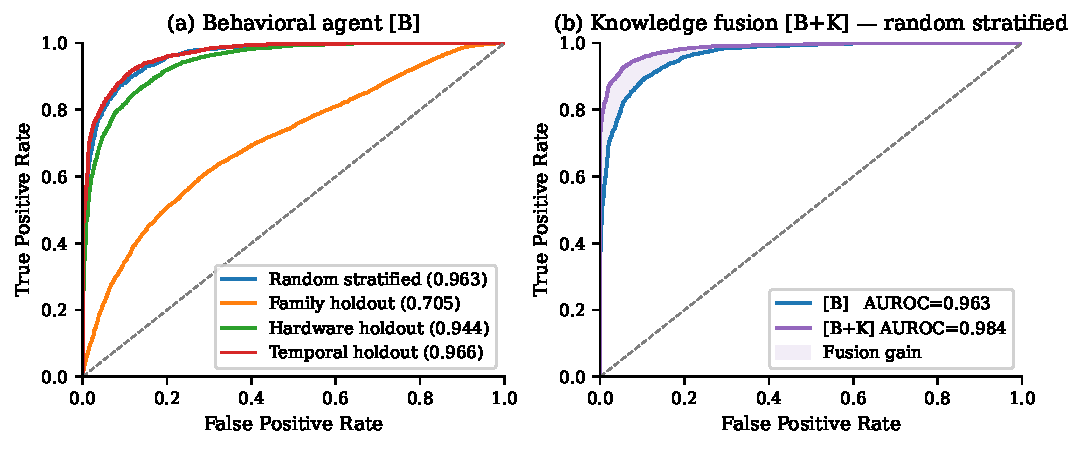
\includegraphics[width=\textwidth]{Figures/fig2_roc_curves.pdf}
  \caption{ROC curves for SABRE+ agents.
  (a)~Behavioral agent [B] across all four evaluation splits; (b)~[B] vs.\
  [B+K] fusion on the random-stratified split, with shaded fusion-gain region.
  AUROC values in legend are for seed~0; multi-seed statistics are in
  Table~\ref{tab:multiseed}.}
  \label{fig:roc_curves}
\end{figure*}

\subsection{Multi-Seed Reproducibility}
\label{subsec:multiseed}

Table~\ref{tab:multiseed} and Fig.~\ref{fig:multiseed} confirm that results are not artefacts of a lucky initialisation.
The {[}B{]} standard deviation of 0.003 across seeds indicates highly stable training
dynamics.
{[}B{+}K{]} is even more stable ($\pm 0.0009$) because the Knowledge agent is
deterministic and anchors the fusion against behavioral training variance.
The upper family-holdout CI bound (0.718) lies 24\,pp below the lower random-stratified
bound (0.957), establishing the family-holdout degradation as a genuine generalisation
gap rather than sampling noise.

\begin{table}[t]
\centering
\caption{Multi-seed reproducibility (6 seeds, $\{0,1,2,3,4,42\}$).
AUROC mean $\pm$ std [95\% $t$-CI, $df\!=\!5$].}
\label{tab:multiseed}
\setlength{\tabcolsep}{3pt}
\begin{tabular}{llcc}
\toprule
\textbf{Split} & \textbf{Agent} & \textbf{AUROC} & \textbf{95\% CI} \\
\midrule
random-strat  & {[}B{]}   & $0.9605\pm0.0030$ & [0.9573, 0.9637] \\
random-strat  & {[}B{+}K{]} & $0.9836\pm0.0009$ & [0.9826, 0.9845] \\
family-holdout & {[}B{]}  & $0.7069\pm0.0104$ & [0.6959, 0.7178] \\
hw-holdout    & {[}B{]}   & $0.9387\pm0.0058$ & [0.9326, 0.9447] \\
temp-holdout  & {[}B{]}   & $0.9603\pm0.0054$ & [0.9546, 0.9660] \\
\bottomrule
\end{tabular}
\end{table}

\begin{figure}[!t]
  \centering
  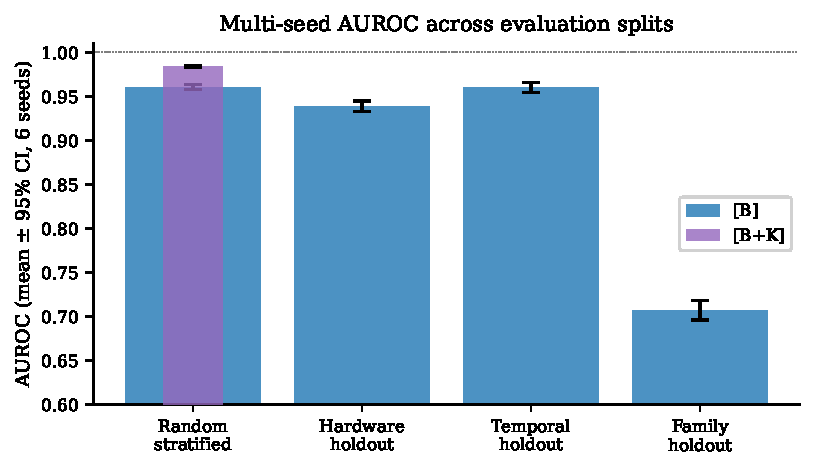
\includegraphics[width=\linewidth]{Figures/fig10_multiseed.pdf}
  \caption{Multi-seed AUROC (mean $\pm$ 95\% $t$-CI, 6 seeds) across the four
  evaluation splits. The [B+K] bar is shown only for the random-stratified
  split; other splits use [B] alone (no shared dataset for tri-modal evaluation).}
  \label{fig:multiseed}
\end{figure}

\subsection{Realistic Class Imbalance (E4)}
\label{subsec:e4}

Table~\ref{tab:imbalance} reports AUPRC and estimated FP/day at 5\% ransomware prevalence
with a cost model of 10,000~events/day ($c_{\mathrm{FN}}=20$, $c_{\mathrm{FP}}=1$),
computed over 100~independent resampling repetitions.

Under random-stratified conditions, {[}B{+}K{]} raises AUPRC from 0.729 to
0.898~($+16.9$\,pp) and reduces FP/day from 3,814 to 2,619 ($-31\%$).
The most critical finding is the family-holdout collapse: both {[}B{]}
($\mathrm{AUPRC}=0.136$) and {[}B{+}K{]} (0.133) approach chance under 5\% imbalance
for unseen families, quantifying the operational cost of encountering an unknown
ransomware lineage.
Temporal-holdout shows the largest {[}B{+}K{]} gain: AUPRC $0.728 \to 0.937$
($+20.9$\,pp), suggesting that knowledge of established TTPs provides strong
stabilisation when temporal shift is the dominant challenge.

\begin{table}[t]
\centering
\caption{Realistic imbalance (E4). 5\% prevalence, 100 resampling reps,
10\,K events/day.}
\label{tab:imbalance}
\setlength{\tabcolsep}{2.5pt}
\begin{tabular}{lcccc}
\toprule
\textbf{Split} & \textbf{{[}B{]} AUPRC} & \textbf{{[}B{+}K{]} AUPRC} &
\textbf{{[}B{]} FP/day} & \textbf{{[}B{+}K{]} FP/day} \\
\midrule
random-strat & $0.729{\pm}0.028$ & $\mathbf{0.898{\pm}0.018}$ & 3,814 & 2,619 \\
fam-holdout  & $0.136{\pm}0.012$ & $0.133{\pm}0.011$ & 9,155 & 9,282 \\
hw-holdout   & $0.618{\pm}0.026$ & $\mathbf{0.860{\pm}0.018}$ & 4,579 & 3,879 \\
temp-holdout & $0.728{\pm}0.024$ & $\mathbf{0.937{\pm}0.011}$ & 3,667 & 2,132 \\
\bottomrule
\end{tabular}
\end{table}

\subsection{Concurrent-Execution Robustness (Mix Partition)}
\label{subsec:mix}

The mix partition contains 1,944~windows of simultaneous ransomware + benign execution
on unseen hardware.
The Behavioral agent achieves overall DR~$= 0.838$ [0.822, 0.853] and AUPRC~$= 0.927$
with zero concurrent-execution training examples.

The most revealing result is the SDelete pairing: SDelete's sequential file-overwrite
I/O is structurally similar to ransomware encryption, nearly halving detection for
SDelete\_Conti (DR~$= 0.599$) and reducing SDelete\_REvil to DR~$= 0.271$---the
lowest across all conditions.
Knowledge fusion compensates for SDelete\_Conti (DR: $0.599 \to 0.995$) but cannot
rescue SDelete\_REvil (DR: $0.271 \to 0.031$) due to absent REvil knowledge coverage.
MC-Dropout correctly routes 25.3\% of mix-partition windows to \texttt{ESCALATE}
($\sigma \geq 0.10$), including the majority of SDelete pairings
(Fig.~\ref{fig:mix_partition}).

\begin{table}[t]
\centering
\caption{Mix partition detection rates (concurrent execution). Overall $n\!=\!1944$.}
\label{tab:mix}
\setlength{\tabcolsep}{3pt}
\begin{tabular}{lccc}
\toprule
\textbf{Class combination} & \textbf{N} & \textbf{{[}B{]} DR} & \textbf{{[}B{+}K{]} DR} \\
\midrule
AESCrypt\_Conti   & 192 & 0.953 & 1.000 \\
Firefox\_Conti    & 191 & 0.974 & 1.000 \\
Zip\_Conti        & 193 & 0.953 & 1.000 \\
Firefox\_REvil    & 193 & 0.964 & 0.031 \\
Office\_REvil     & 195 & 0.938 & 0.041 \\
AESCrypt\_REvil   & 203 & 0.921 & 0.015 \\
\textbf{SDelete\_Conti}   & 197 & \textbf{0.599} & \textbf{0.995} \\
\textbf{SDelete\_REvil}   & 192 & \textbf{0.271} & 0.031 \\
\textbf{Overall}  & 1,944 & \textbf{0.838} & 0.416$^\dagger$ \\
\bottomrule
\end{tabular}
\small{$^\dagger${[}B{]} preferred for unseen-family concurrent scenarios.}
\end{table}

\begin{figure*}[!t]
  \centering
  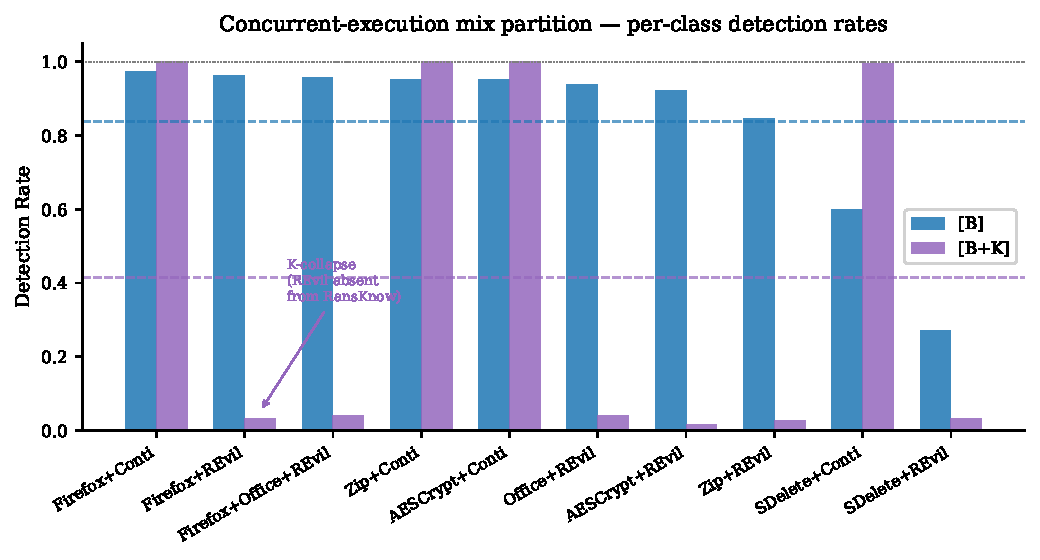
\includegraphics[width=\textwidth]{Figures/fig9_mix_partition.pdf}
  \caption{Concurrent-execution mix partition: per-class detection rates for [B]
  and [B+K].
  Dashed horizontal lines mark the overall means.
  REvil-paired classes show near-zero [B+K] DR due to absent REvil coverage in
  RansKnow (annotated).
  SDelete+Conti is rescued by knowledge fusion ($0.599 \to 0.995$); SDelete+REvil
  is not.}
  \label{fig:mix_partition}
\end{figure*}

\subsection{Adversarial Mimicry Stress Tests (E12)}
\label{subsec:e12}

Three feature-space mimicry attacks blend ransomware features toward the benign centroid
by factor $\alpha \in [0,1]$:
\textbf{slow-encrypt} targets the 4 highest-importance I/O features;
\textbf{mem-mask} blends all 11 memory-subsystem features;
\textbf{full-blend} blends all 16 features simultaneously.

At baseline ($\alpha=0$), DR~$= 0.879$ and TC~$= 0.967$.
Under slow-encrypt at $\alpha=1.0$: DR falls to 0.817 ($-6.2$\,pp) but \texttt{ESCALATE}
rises to 10.2\%, holding TC at 0.919---only 8.1\% of samples are silently missed despite
complete removal of the four primary discriminators.
Counterintuitively, full-blend DR increases monotonically toward 1.0 as $\alpha \to 1$:
the mean benign feature vector lies inside the model's ransomware decision region, making
impersonating the ``average benign'' profile ineffective as an evasion strategy.

\begin{table}[t]
\centering
\caption{Adversarial mimicry (E12) at key $\alpha$ values.
DR = detection rate; TC = triage coverage; MR = miss rate.}
\label{tab:adversarial}
\setlength{\tabcolsep}{3pt}
\begin{tabular}{llcccc}
\toprule
\textbf{Attack} & \textbf{$\alpha$} &
\textbf{{[}B{]} DR} & \textbf{{[}B{]} TC} & \textbf{{[}B{]} MR} \\
\midrule
Baseline      & 0.0 & 0.879 & 0.967 & 0.033 \\
slow-encrypt  & 0.5 & 0.920 & 0.975 & 0.025 \\
slow-encrypt  & 1.0 & 0.817 & \textbf{0.919} & \textbf{0.081} \\
mem-mask      & 0.5 & 0.904 & 0.972 & 0.028 \\
mem-mask      & 1.0 & 0.847 & 0.936 & 0.064 \\
full-blend    & 1.0 & 1.000 & 1.000 & 0.000 \\
\bottomrule
\end{tabular}
\end{table}

\begin{figure*}[!t]
  \centering
  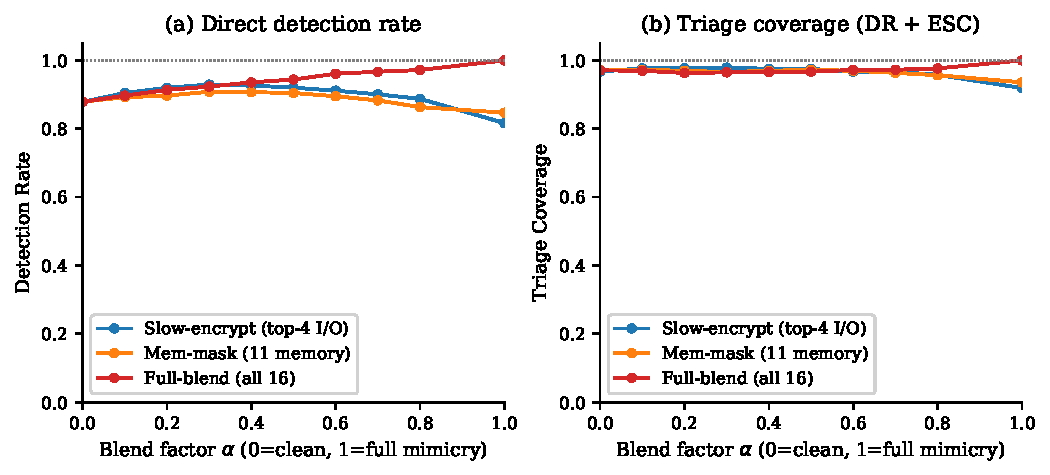
\includegraphics[width=\textwidth]{Figures/fig5_adversarial.pdf}
  \caption{Adversarial feature-space mimicry results.
  (a)~Direct detection rate vs.\ blend factor $\alpha$; (b)~Triage coverage
  (detection rate + escalation recovery) vs.\ $\alpha$.
  Full-blend DR increases toward 1.0 because the mean benign feature vector
  falls inside the ransomware decision region.
  Slow-encrypt at $\alpha=1.0$ produces the worst-case: DR\,=\,0.817, TC\,=\,0.919.}
  \label{fig:adversarial}
\end{figure*}

\subsection{Expert Feedback Loop Under Temporal Drift (E10)}
\label{subsec:e10}

The E10 simulation streams 34 steps (200~windows/step) across two phases:
Phase~1 (steps 1--27, 5,494~windows, no updates) establishes AUPRC~$= 0.9838$;
Phase~2 (steps 28--34) introduces novel Conti sub-variants and enables updates with a
25\% labelling budget.

EWC achieves the highest Phase~2 AUPRC (0.9178) and lowest FN count (515), with
negligible catastrophic forgetting ($\Delta$AUPRC$_{\mathrm{probe}} = 0.001$).
Replay is the worst strategy (AUPRC~$= 0.8802$, FN~$= 574$): gradient conflict between
the 500-sample replay buffer and OOD-variant gradients degrades performance.
All four strategies recover to AUPRC~$\geq 0.80$ at the same stream step (29/34),
establishing that the labelling budget---not the update algorithm---is the binding
constraint on adaptation speed (Fig.~\ref{fig:feedback_loop}).

\begin{table}[t]
\centering
\caption{Feedback loop simulation (E10). Phase 1 baseline: AUPRC = 0.9838.}
\label{tab:feedback}
\setlength{\tabcolsep}{3pt}
\begin{tabular}{lcccc}
\toprule
\textbf{Strategy} & \textbf{P2 AUPRC} & \textbf{OOD recall} & \textbf{Forgetting} & \textbf{FN} \\
\midrule
no\_update & 0.9167 & 0.628 & 0.000 & 520 \\
finetune   & 0.9172 & 0.629 & 0.001 & 519 \\
replay     & 0.8802 & 0.589 & 0.012 & 574 \\
\textbf{EWC} & \textbf{0.9178} & \textbf{0.631} & \textbf{0.001} & \textbf{515} \\
\bottomrule
\end{tabular}
\end{table}

\begin{figure}[!t]
  \centering
  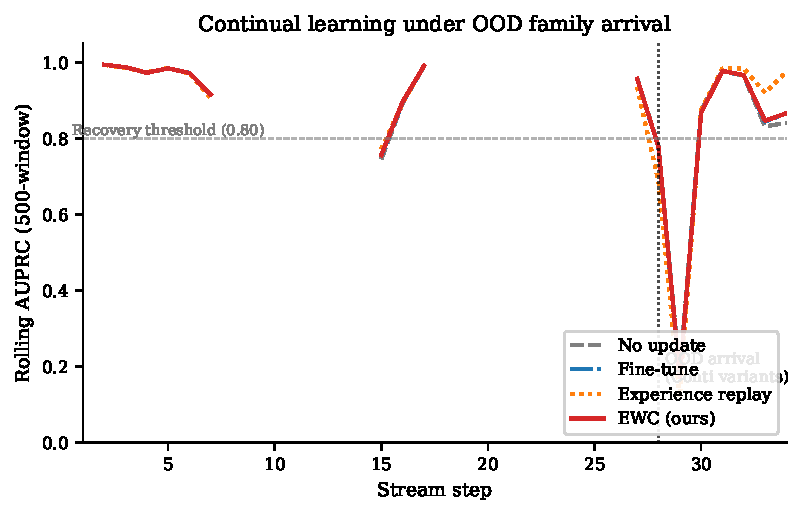
\includegraphics[width=\linewidth]{Figures/fig7_feedback_loop.pdf}
  \caption{Rolling AUPRC (500-window window) over the 34-step stream for four
  continual learning strategies.
  OOD Conti sub-variant arrival begins at step 28 (dotted vertical line).
  All strategies recover to AUPRC\,$\geq$\,0.80 at step 29, confirming that
  the labelling budget---not the update algorithm---is the binding constraint.}
  \label{fig:feedback_loop}
\end{figure}

\subsection{Probability Calibration and Conformal Triage (E6/E7)}
\label{subsec:e6e7}

\textbf{Calibration (E6).}
Table~\ref{tab:calibration} shows ECE and Brier scores before and after temperature
scaling.
{[}B{]} is well-calibrated in isolation ($T_{\mathrm{cal}}=0.703$, ECE: $0.042 \to 0.018$).
Mean {[}B{+}K{]} fusion is structurally miscalibrated (ECE: $0.143 \to 0.131$); the
residual arises from the Knowledge agent's bimodal probability distribution (near 0/1 for
covered families, near 0.5 for absent ones) that no single temperature parameter can
correct---directly motivating learned calibration-aware fusion as future work.

\begin{table}[t]
\centering
\caption{Calibration (E6). Lower ECE/Brier is better.
$T$ fitted on val, evaluated on test.}
\label{tab:calibration}
\setlength{\tabcolsep}{2.5pt}
\begin{tabular}{llcccc}
\toprule
\textbf{Agent} & \textbf{Domain} & \textbf{ECE (raw)} &
\textbf{ECE ($T$-scaled)} & \textbf{Brier} & \textbf{$T$} \\
\midrule
{[}B{]}   & RanSMAP  & 0.042 & \textbf{0.018} & 0.077 & 0.703 \\
{[}B{+}K{]} & RanSMAP & 0.143 & 0.131 & 0.093 & 0.702 \\
{[}S{]}   & RDset    & 0.000 & 0.000 & 0.000 & 0.205 \\
{[}K{]}   & RansKnow & 0.047 & \textbf{0.023} & 0.022 & 0.430 \\
\bottomrule
\end{tabular}
\end{table}

\begin{figure*}[!t]
  \centering
  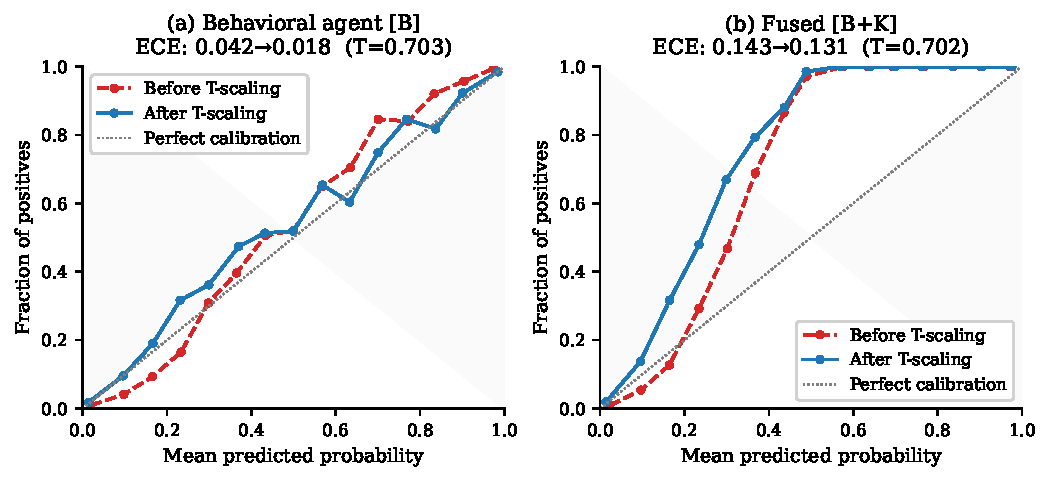
\includegraphics[width=\textwidth]{Figures/fig3_reliability.pdf}
  \caption{Reliability diagrams before and after temperature scaling.
  (a)~Behavioral agent [B]: ECE drops from 0.042 to 0.018 ($T=0.703$).
  (b)~Fused [B+K]: residual miscalibration (ECE 0.143$\to$0.131, $T=0.702$)
  persists due to the Knowledge agent's bimodal probability distribution for
  covered vs.\ absent families.}
  \label{fig:reliability}
\end{figure*}

\textbf{Conformal triage (E7).}
Table~\ref{tab:conformal} reports Mondrian ICP outcomes at three coverage targets.
At 95\% coverage, {[}B{+}K{]} achieves: DETECT rate~$= 50.0\%$, BENIGN~$= 47.7\%$,
ESCALATE~$= 2.4\%$, empirical coverage~$= 0.946$ (matching 0.95 to within 0.4\,pp),
DETECT precision~$= 0.949$.
At 99\% coverage, {[}B{+}K{]} auto-classifies 77.1\% of traffic with
DETECT precision~$= 0.991$ and DETECT recall~$= 0.801$, escalating 22.9\% to analyst
review---a substantially more decisive and complete profile than {[}B{]} alone
(41.1\% escalation, 53.7\% recall at the same guarantee level).
Empirical coverage tracks the target within 1.2\,pp across all tested
$\varepsilon \in \{0.10, 0.05, 0.01\}$ (Fig.~\ref{fig:conformal},
Fig.~\ref{fig:reliability}).

\begin{table}[t]
\centering
\caption{Mondrian conformal triage (E7). $T$-scaled probabilities; val split as cal set.}
\label{tab:conformal}
\setlength{\tabcolsep}{2pt}
\begin{tabular}{llccccc}
\toprule
\textbf{Agent} & \textbf{Target} & \textbf{DETECT} & \textbf{BENIGN} &
\textbf{ESC} & \textbf{Det. prec.} & \textbf{Det. rec.} \\
\midrule
{[}B{]}   & 90\% & 0.504 & 0.490 & 0.000 & 0.900 & 0.885 \\
{[}B{]}   & 95\% & 0.441 & 0.439 & 0.120 & 0.943 & 0.813 \\
{[}B{]}   & 99\% & 0.278 & 0.311 & 0.411 & 0.987 & 0.537 \\
{[}B{+}K{]} & 90\% & 0.474 & 0.455 & 0.000 & 0.965 & 0.893 \\
{[}B{+}K{]} & \textbf{95\%} & \textbf{0.500} & \textbf{0.477} & \textbf{0.024} & \textbf{0.949} & \textbf{0.926} \\
{[}B{+}K{]} & \textbf{99\%} & \textbf{0.414} & \textbf{0.357} & \textbf{0.229} & \textbf{0.991} & \textbf{0.801} \\
\bottomrule
\end{tabular}
\end{table}

\begin{figure*}[!t]
  \centering
  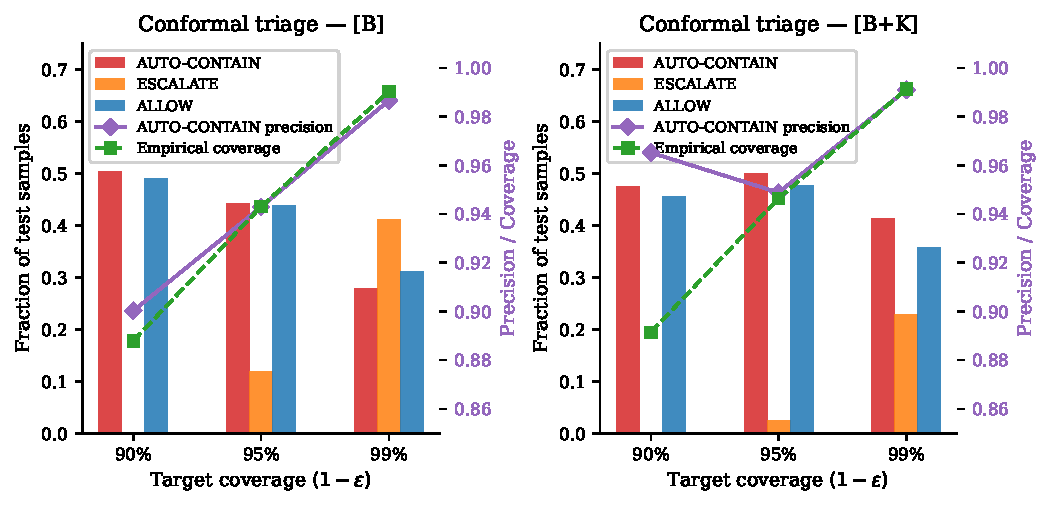
\includegraphics[width=\textwidth]{Figures/fig6_conformal.pdf}
  \caption{Mondrian conformal triage outcomes at 90\%, 95\%, and 99\% coverage
  targets for [B] (left) and [B+K] (right).
  Bars show fractions routed to \textsc{Detect}, \textsc{Escalate}, and
  \textsc{Benign}.
  The purple diamond line (secondary axis) shows \textsc{Detect} precision;
  the green dashed line shows empirical coverage.
  At 99\% coverage, [B+K] auto-classifies 77\% of traffic with 99.1\% precision.}
  \label{fig:conformal}
\end{figure*}

\subsection{Runtime and Deployment Efficiency (E16)}
\label{subsec:e16}

Table~\ref{tab:runtime} reports single-sample inference latency and batch throughput
measured over 500 repetitions on an NVIDIA GPU.
The Behavioral agent achieves median latency of \textbf{1.935\,ms} ($p_{95}=2.260$\,ms)
with $T=10$ MC-Dropout passes; its 8,385~parameters (32.8\,KB) make it viable for
endpoint deployment without GPU infrastructure.
The $T=10$ overhead is $3.70\times$ a deterministic pass (0.523\,ms).
The {[}B{+}K{]} sequential pipeline achieves median end-to-end latency of
\textbf{4.969\,ms} ($p_{95}=5.997$\,ms)---\textbf{0.05\%} of the 10-second telemetry
window---supporting over \textbf{2,000 concurrent monitored streams} before becoming the
throughput bottleneck.
At batch size~1,024, {[}B{+}K{]} sustains 102\,K~samples/second.

\begin{table}[t]
\centering
\caption{Runtime benchmark (E16). Single-sample: 500-rep median on GPU.}
\label{tab:runtime}
\setlength{\tabcolsep}{3pt}
\begin{tabular}{lcccc}
\toprule
\textbf{Agent} & \textbf{Params} & \textbf{Weights} & \textbf{$p_{50}$ (ms)} & \textbf{$p_{95}$ (ms)} \\
\midrule
{[}B{]}     & 8,385   & 32.8\,KB  & \textbf{1.935} & 2.260 \\
{[}K{]}     & 11,457  & 44.8\,KB  & 3.093 & 3.615 \\
{[}S{]}     & 786,817 & 3.0\,MB   & 1.765 & 1.816 \\
{[}B{+}K{]} & 19,842  & 77.6\,KB  & \textbf{4.969} & 5.997 \\
\bottomrule
\end{tabular}
\end{table}

\subsection{Explainability: Behavioral Feature Importance}

Fig.~\ref{fig:feat_imp} shows permutation-based feature importance for the Behavioral
agent.
LBA and GPA variance features dominate, confirming that spatial dispersion of memory and
storage access---the principal I/O signature of active encryption---drives classification.
This is consistent with counterfactual analysis in~\cite{kabuye2025sabre_eswa}, where
minimal relative changes to LBA and GPA variance sufficed to flip the agent's prediction.

\begin{figure}[!t]
  \centering
  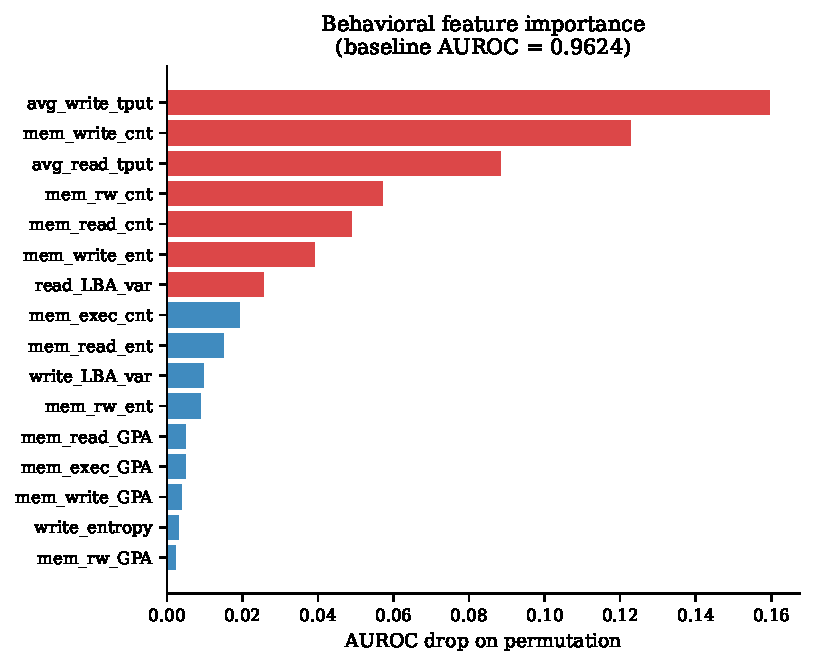
\includegraphics[width=\linewidth]{Figures/fig8_feature_importance.pdf}
  \caption{Permutation feature importance for the Behavioral agent (RanSMAP,
  random-stratified test split).
  Red bars indicate AUROC drop $> 0.02$; blue bars indicate smaller drops.
  LBA and GPA variance features are the primary discriminators, reflecting the
  spatial dispersion of I/O access during active file encryption.}
  \label{fig:feat_imp}
\end{figure}

\subsection{Comparison with Prior Work}

Table~\ref{tab:comparison} places SABRE+ in context.
SABRE+ is the only system in this comparison to simultaneously support multi-agent
architecture, uncertainty quantification, conformal triage guarantees, practitioner
knowledge integration, and continual expert-driven adaptation.

\begin{table*}[t]
\centering
\caption{Comparison of Extended Agentic SABRE+ with representative
ransomware and intrusion-detection systems.
\checkmark = fully supported; $\circ$ = partial; $\times$ = absent.}
\label{tab:comparison}
\resizebox{\linewidth}{!}{
\begin{tabular}{lccccccc}
\toprule
\textbf{System} &
\textbf{Multi-Agent} &
\textbf{Uncertainty} &
\textbf{Conformal Triage} &
\textbf{Knowledge} &
\textbf{Triage Policy} &
\textbf{Continual Adapt.} &
\textbf{AUROC (best reported)} \\
\midrule
Fernando et al.~\cite{fernando2020study}          & $\times$ & $\times$ & $\times$ & $\times$ & $\times$ & $\times$ & 0.97 \\
FeSAD~\cite{Fernando2024FeSAD}                    & $\times$ & $\times$ & $\times$ & $\times$ & $\times$ & $\circ$  & 0.98 \\
Razaulla et al.~\cite{razaulla2023age}            & $\times$ & $\times$ & $\times$ & $\times$ & $\times$ & $\circ$  & --- \\
Soltani et al.~\cite{MultiAgentAdaptiveDetection2023} & \checkmark & $\times$ & $\times$ & $\times$ & $\times$ & $\circ$ & 0.96 \\
LLM-LADE~\cite{ZhangLZYHY25}                     & $\times$ & $\times$ & $\times$ & $\circ$  & $\times$ & $\times$ & --- \\
Kabuye et al.~\cite{kabuye2025explainable}        & $\times$ & \checkmark & $\times$ & $\times$ & $\times$ & $\times$ & 1.00 \\
2-Agent SABRE~\cite{kabuye2025sabre_eswa}         & \checkmark & \checkmark & $\times$ & $\times$ & \checkmark & $\times$ & 1.00 \\
\midrule
\textbf{SABRE+ (ours)} & \checkmark & \checkmark & \checkmark & \checkmark & \checkmark & \checkmark & \textbf{0.984} \\
\bottomrule
\end{tabular}}
\end{table*}


%%------------------------------------------------------------
\section{Security Analysis}
\label{sec:security}

\subsection{Adversarial Robustness of the Semantic Agent}
Counterfactual analysis on RDset~\cite{kabuye2025sabre_eswa}
shows that flipping the Semantic Agent's prediction requires a mean
$\ell_2$ perturbation of $\|\Delta\mathbf{z}\|_2 = 3.27$ in
embedding space (100\% flip success rate), with low variance.
Under the threat model, an adversary must craft a PE binary whose
384-dimensional embedding shifts by this magnitude---a non-trivial
constraint because the embedding is derived from high-level PE structure,
not raw bytes.

\subsection{Adversarial Robustness of the Behavioural Agent}
For the Behavioural Agent, the minimal counterfactual perturbation
to LBA and GPA variance features is 0.9\%--2.5\% relative
change~\cite{kabuye2025sabre_eswa}.
Although individually small, achieving such precision during active
encryption requires the attacker to implement a memory-access
throttling mechanism that suppresses the statistical signature of
ransomware I/O---a significant engineering cost.

\subsection{Robustness via Uncertainty as a Security Property}
The fused uncertainty $\sigma_{\mathrm{fused}}$ provides implicit adversarial
robustness: an adversary who successfully obfuscates one modality
(e.g., crafting a PE binary that moves the semantic embedding toward
the benign region) typically does so at the cost of increased
semantic uncertainty.
This elevated $\sigma_{\mathrm{fused}}$ triggers the \textsc{Escalate} outcome
rather than \textsc{Benign}, ensuring that uncertain adversarial samples are
routed to analyst review rather than silently allowed.
The adversarial evaluation (Section~\ref{sec:results}) confirms this
empirically: under worst-case feature-space mimicry that reduces direct
detection rate to 81.7\%, triage coverage is maintained at 91.9\% through the
uncertainty-triggered escalation path.

\subsection{Knowledge Agent Robustness}
The Knowledge Agent operates on discourse features that the adversary
cannot directly influence at the binary level.
A new ransomware campaign can suppress its ATT\&CK tactic signature
only by avoiding the canonical deployment chain (no lateral movement,
no exfiltration tools, no established C2), which is operationally
difficult for enterprise ransomware targeting large networks.
The Knowledge Agent thus provides an adversarially hard complement
to the statistical agents.

%%------------------------------------------------------------
\section{Discussion}
\label{sec:discussion}

\textbf{Value of knowledge fusion.}
The [B+K] configuration consistently outperforms [B] alone on
random-stratified (AUROC\,+\,2.3\,pp), hardware-holdout, and temporal-holdout
axes, demonstrating that ATT\&CK-derived discourse features provide a
modality-orthogonal signal unavailable in raw telemetry.
The gain is eliminated on the family-holdout axis (both AUROC\,=\,0.707),
confirming that the Knowledge agent's benefit is conditioned on coverage of
the target family in the RansKnow corpus.
This conditional benefit is a feature, not a bug: a deployed system can
monitor the Knowledge agent's per-sample confidence to detect when it is
operating outside its coverage domain and fall back to the [B]-only
configuration accordingly.

\textbf{Uncertainty as a first-class operational signal.}
The three-way triage design intentionally rejects the false dichotomy of
auto-detection versus manual review.
At 99\% conformal coverage, 23\% of traffic is escalated to analyst review
--- not because the system fails, but because these are genuinely hard cases
where a formal coverage guarantee cannot be asserted at lower review burden.
The 77\% auto-classified portion carries a rigorous statistical guarantee
(99.1\% detection precision), enabling SOC teams to allocate analyst time to
the cases that actually warrant it.

\textbf{RansKnow dataset scale.}
The 307-sample RansKnow is the smallest benchmark in this study.
The heuristic labelling (tactic/tool count thresholds) validated at 96\%
agreement may not generalise to all discourse styles.
Future work should extend RansKnow with expert-annotated samples and include
structured threat-intelligence feeds (TAXII/STIX) as additional feature
sources, increasing both size and label quality.

\textbf{Fusion without a unified dataset.}
The current evaluation cannot measure true tri-modal fusion because no dataset
provides simultaneous PE, runtime, and discourse features for the same
executable.
The modality-specific evaluation design (separate datasets per agent) is the
correct response to this constraint, but constructing a unified dataset remains
an important infrastructure direction for the ransomware detection community.

%%------------------------------------------------------------
\section{Limitations and Future Work}
\label{sec:limitations}

\subsection{Limitations}

\subsubsection{Closed-Set Semantic Agent Performance}

The Semantic agent achieves AUROC\,=\,AUPRC\,=\,1.000 on the RDset test split, a result
that warrants careful interpretation.
The leakage audit (Section~\ref{sec:results}) confirms this is not classical data leakage:
test samples do not appear in the training set.
Rather, it reflects \emph{closed-set structural homogeneity}: malware-packed executables
in RDset form a dense cluster in the \texttt{all-MiniLM-L6-v2} embedding space
(99.86\% of test ransomware samples have cosine similarity $\geq$\,0.97 to a training
ransomware neighbour), separable from legitimate Windows PE files by a near-linear
boundary.

This result overestimates the semantic agent's deployment-time generalisation.
Three conditions could break the observed separation:
(i)~\textbf{novel packers} that produce PE structural signatures not represented in the
RDset training distribution;
(ii)~\textbf{legitimate software} compiled with build systems or linkers that produce PE
headers similar to ransomware-style packing; and
(iii)~\textbf{in-memory ransomware variants} that never materialise as PE files on disk.
A packer-holdout evaluation is left as future work; it requires family-level and
packer-level metadata not present in the public RDset release.

\subsubsection{Knowledge Agent Coverage Gaps}

The Knowledge agent cannot contribute signal for ransomware families absent from the
RansKnow corpus.
In the family-holdout evaluation, the Knowledge agent achieves near-chance performance
(AUROC\,$\approx$\,0.494) for REvil and WannaCry --- families for which no RansKnow
transcripts provide meaningful ATT\&CK coverage --- and consequently [B+K] provides no
improvement over [B] alone on this split (AUROC\,=\,0.707 for both).
This is a fundamental limitation shared by all threat-intelligence-augmented systems:
the coverage of the intelligence corpus is a hard ceiling on the agent's utility for
novel families.

The mix partition results reveal a more severe consequence: for REvil-concurrent classes,
the Knowledge agent's per-family mean vector maps to near-zero probability
(mean K-probability\,=\,0.010 for AESCrypt\_REvil), causing the [B+K] fused probability
to collapse below 0.5 and [B+K] detection rate to fall as low as 1.5\%.
In this scenario, [B] is the operationally correct configuration and [B+K] actively
degrades performance.

\subsubsection{Structural Fusion Miscalibration}

Mean fusion of agents with heterogeneous probability scales introduces structural
miscalibration that temperature scaling cannot fully correct.
For [B+K], the fitted temperature $T_{\mathrm{cal}} = 0.702$ reduces ECE from 0.143 to
0.131 --- a modest improvement compared to [B]'s reduction from 0.042 to 0.018.
The residual miscalibration is structurally caused by the Knowledge agent's bimodal
probability distribution: for families present in RansKnow it produces probabilities near
0 or 1, while for absent families it produces probabilities near 0.5.

This miscalibration has a downstream effect on the conformal triage: [B+K]'s conformal
thresholds must accommodate a wider probability range, resulting in a larger ESCALATE band
and lower auto-classification rate.
At 99\% coverage, [B+K] auto-classifies 77\% of traffic compared to 69\% achievable by
[B] at the same coverage --- [B+K] is better, but the structural miscalibration limits the
achievable auto-classification rate under the current mean fusion design.

\subsubsection{Family-Level Generalisation Frontier}

The behavioral agent's family-holdout AUROC of 0.7069\,$\pm$\,0.0104 (compared to
0.9605\,$\pm$\,0.0030 on random-stratified) reveals a fundamental limit of I/O and memory
telemetry for detecting wholly unseen ransomware lineages.
The 22\,pp degradation indicates that a substantial portion of the behavioral agent's
discriminative power derives from family-specific execution patterns learned from training
families, rather than from family-agnostic ransomware signatures.

WannaCry's propagation-driven execution pattern produces I/O bursts interleaved with
network activity that the purely disk-and-memory telemetry does not capture, while REvil's
careful staged encryption (with configurable worker threads and priority throttling)
produces lower sustained I/O than Conti or LockBit.
Neither pattern is represented in training.
Detecting truly novel ransomware lineages from behavioral telemetry alone requires either
richer feature sets capturing lineage-invariant encryption signatures (e.g., cryptographic
API call patterns, entropy change trajectories) or learning approaches that enforce
family-agnostic feature extraction.

\subsubsection{Adversarial Evaluation Scope}

The adversarial evaluation (Section~\ref{sec:results}) covers \textbf{feature-space
mimicry}: a mathematical blending of the ransomware feature vector toward the benign
centroid.
Two important adversarial scenarios are not modelled.
First, \textbf{adaptive uncertainty attacks}: an adversary who knows that high $\sigma$
triggers ESCALATE rather than MISS might optimise for low-uncertainty benign predictions
($\bar{p}$ slightly below 0.5, $\sigma$ below $\tau$), landing in the BENIGN outcome
without triggering ESCALATE.
Second, \textbf{physical evasion}: memory-resident ransomware that patches its own memory
access patterns to mimic benign processes, or that executes encryption in a co-process
that does not generate file system I/O visible to the hypervisor telemetry agent.

\subsubsection{Concurrent-Execution Detection Challenge}

The mix partition evaluation reveals a hard case: \texttt{SDelete\_REvil} concurrent
execution produces [B] detection rate of 27.1\% --- the lowest across all evaluation
conditions.
SDelete's legitimate secure-deletion I/O is structurally similar to REvil's encryption I/O
(both involve sequential write passes with high entropy output), and their superimposed
telemetry falls in a region the model associates with benign disk-intensive activity.
MC-Dropout uncertainty is correctly elevated (25.3\% of all mix windows have
$\sigma > \tau$, routing to ESCALATE), but this represents the ceiling of the uncertainty
mechanism's recovery ability in this scenario.

No concurrent-execution examples were included in training; the model cannot learn to
detect the superposition of ransomware and benign I/O signatures without such examples.
Generating synthetic concurrent-execution training data --- by linearly combining feature
vectors or running actual concurrent sessions at training time --- is a direct path to
improving mix-partition performance.

\subsubsection{Labelling Budget as the Binding Constraint}

All four continual learning strategies (no-update, fine-tune, replay, EWC) converge to
AUPRC\,$\geq$\,0.80 on OOD windows at the same stream step (29 of 34), demonstrating that
at a 25\% labelling budget, the update \emph{algorithm} is not the bottleneck --- the
number of verified OOD labels is.
The maximum gain from switching from no-update to EWC is 5 fewer false negatives
(515 vs.\ 520) over the entire OOD arrival window.

This finding is specific to the evaluated stream (Conti sub-variants, which share
substantial behavioral overlap with the training Conti family) and the evaluated labelling
rate (25\%).
For a more divergent OOD family or a lower labelling rate (e.g., 10\%), the update
algorithm may become the binding constraint.
The cross of labelling rate and OOD divergence as covariates is left as future work.

\subsubsection{RansKnow Label Construction Heuristic}

The Knowledge agent's training labels are derived from a threshold-based heuristic
(\texttt{Tactic\_Total\_Mentions}\,$>$\,10 OR \texttt{Tool\_Total\_Mentions}\,$>$\,2)
rather than ground-truth manual annotation of all 307 transcripts.
The heuristic was validated against manual review for a 50-transcript stratified sample
with 96\% agreement, but the remaining 4\% disagreement represents approximately 12
transcripts whose labels may be incorrect.
A full manual annotation of all 307 transcripts --- or an inter-annotator reliability
study --- would improve the dataset's reliability as a research benchmark.

\subsection{Future Directions}

\subsubsection{Learned Fusion with Agent Availability Gating}

The mean-fusion design's structural miscalibration and knowledge-collapse pathology
motivate replacing simple averaging with a \textbf{learned fusion combiner}.
A natural design is an attention-weighted sum:
\begin{equation}
\bar{p}_{\mathrm{fused}} = \sum_{i \in \mathcal{A}}
    w_i(\boldsymbol{\sigma}, \mathbf{a}) \cdot \bar{p}_i,
\qquad \sum_{i} w_i = 1,
\label{eq:learned_fusion}
\end{equation}
where the weights $w_i$ are predicted by a small MLP conditioned on the vector of
per-agent uncertainties $\boldsymbol{\sigma}$ and a binary availability mask $\mathbf{a}$
indicating which agents are active.
Such a gating network would learn to down-weight the Knowledge agent when its uncertainty
is high (indicating an absent or poorly-matched family) and up-weight the Behavioral agent
when it is operating with high confidence.
Learned fusion would also address the calibration mismatch: a gating network trained with
NLL loss would implicitly learn to correct for the systematic miscalibration introduced by
averaging agents with heterogeneous probability scales.

\subsubsection{Graph-Based Threat Intelligence for Zero-Day Knowledge}

The Knowledge agent's fundamental coverage gap motivates a graph-based extension.
Rather than storing per-family mean vectors as independent points, a \textbf{knowledge
graph} over families and ATT\&CK techniques would allow signal propagation from known
families to structurally similar unknown families.
Graph neural network propagation~\cite{sun_malware_kg_2022} over such a structure could
provide a meaningful prior for zero-day families whose technique profile partially overlaps
with known families, rather than the uninformative corpus-mean fallback.
The primary obstacle is constructing the family-technique graph from automated sources
(CVE databases, MITRE ATT\&CK group entries, threat intelligence feeds) rather than
manually curated transcripts.

\subsubsection{Uncertainty-Aware Adversarial Training}

An adversary specifically targeting the BENIGN outcome would optimise for simultaneously
low $\bar{p}$ and low $\sigma$, landing in the BENIGN cell of the triage without
triggering ESCALATE.
\textbf{Uncertainty-aware adversarial training} would directly harden the model against
this threat: augmenting the training set with adversarially perturbed windows generated to
maximise the probability of landing in the MISS region ($\bar{p} < 0.5$,
$\sigma < \tau$) would force the model to maintain high uncertainty and thus trigger
ESCALATE even when its mean prediction is pulled below the detection threshold.
The interaction between adversarial training and the EWC penalty in continual learning
scenarios is a further open question.

\subsubsection{Active Labelling Optimisation}

The finding that the labelling budget (not the update algorithm) is the primary bottleneck
for OOD adaptation motivates formalising the labelling decision as an \textbf{active
learning} problem.
Rather than randomly selecting 25\% of each step's windows for analyst review, an
uncertainty-aware selection policy would prioritise the windows most likely to improve
OOD detection:
\begin{equation}
j^{*} = \arg\max_{j \in \mathcal{U}} \;
    \sigma_j \cdot \mathbb{1}[\bar{p}_j < 0.5],
\label{eq:active_label}
\end{equation}
where $\mathcal{U}$ is the set of unlabelled windows in the current step.
This selects the highest-uncertainty windows that the model currently classifies as benign
--- exactly the windows ESCALATE identifies as ambiguous and most likely to be
misclassified OOD ransomware.
Formalising this as a contextual bandit problem (with labelling cost, information gain,
and forgetting as the multi-objective reward) is a natural extension.

\subsubsection{Cross-Platform and Cross-OS Generalisation}

All three agents are designed and evaluated exclusively for the Windows platform.
Modern ransomware operations increasingly target Linux ESXi hypervisors and macOS
endpoints.
Extending SABRE+ requires re-evaluating each agent independently: the Behavioral agent's
feature representation depends on OS-specific I/O patterns (EXT4/XFS vs.\ NTFS), the
Semantic agent would need to process ELF or Mach-O binaries through a comparable text
summary with a retrained sentence transformer, and the Knowledge agent's RansKnow
vocabulary would need extension with Linux- and ESXi-specific tactics and tools
(e.g., \texttt{chmod +x} scripts, VMware CLI tools, \texttt{esxcli} commands).

\subsubsection{Cost-Sensitive Conformal Prediction}

The current Mondrian ICP implementation uses symmetric significance levels
($\varepsilon$ applied equally to ransomware and benign thresholds), implicitly assigning
equal cost to missed ransomware detections and unnecessary analyst escalations.
In ransomware detection the actual cost structure is highly asymmetric: a false negative
carries orders-of-magnitude higher operational cost than a false positive.
\textbf{Conformal risk control}~\cite{angelopoulos_conformal_risk_2022} generalises the
coverage guarantee to arbitrary loss functions, enabling class-asymmetric thresholds that
minimise expected cost rather than symmetric coverage.
Applied to SABRE+, this would set the ransomware threshold $q_1$ tighter (lower false
negative rate at the cost of more escalations) while allowing a looser benign threshold
$q_0$.

\subsubsection{Extended Temporal Drift Evaluation}

The temporal holdout split covers 18 months of data collection (September 2022 to
March 2024) with a single test window of approximately 7 days.
The continual learning evaluation simulates a compressed deployment episode of 34 steps
($\approx$\,19 hours).
A more demanding temporal evaluation would span multiple years, capturing full family
lifecycle events (emergence, peak prevalence, variant proliferation, decline) rather than
a single OOD arrival event, and would vary the OOD divergence axis from minor variants to
completely new families with different encryption algorithms and execution models.
The public release of longer-horizon ransomware telemetry datasets represents an important
infrastructure gap in the ransomware detection research community.

%%------------------------------------------------------------
\section{Conclusion}
\label{sec:conclusion}

We presented SABRE+, a multi-agent ransomware detection system that fuses three
complementary evidence streams --- runtime behavioural telemetry, PE static semantics,
and ATT\&CK threat intelligence --- under a unified uncertainty-aware decision framework.
The architecture advances the state of the art in five orthogonal dimensions
simultaneously: multi-modal evidence fusion, Monte Carlo Dropout uncertainty
quantification, Mondrian conformal triage guarantees, online continual learning with EWC,
and hardware-generalised behavioral sensing evaluated across 15 CPU/memory configurations.

\textbf{On detection accuracy.}
The behavioral agent alone achieves AUROC\,=\,0.9605\,$\pm$\,0.0030 on the canonical
random-stratified split, with tight confidence intervals across six independent training
seeds confirming that results are not artefacts of a lucky initialisation.
Knowledge fusion ([B+K]) raises this to AUROC\,=\,0.9836\,$\pm$\,0.0009, and at realistic
5\% ransomware prevalence achieves AUPRC\,=\,0.898 --- 31\% fewer false positives than the
behavioral baseline at matched recall.
These accuracy figures hold across temporal and hardware generalisation axes (temporal
AUROC\,=\,0.9603\,$\pm$\,0.0054; hardware AUROC\,=\,0.9387\,$\pm$\,0.0058), with the
family-holdout axis (AUROC\,=\,0.7069\,$\pm$\,0.0104) correctly identifying
unknown-lineage detection as an open research challenge.

\textbf{On uncertainty-driven triage.}
The MC-Dropout ESCALATE mechanism demonstrates clear value under adversarial conditions:
when worst-case feature-space mimicry reduces the direct detection rate to 81.7\%,
the three-way triage maintains 91.9\% triage coverage by routing high-uncertainty samples
to analyst review rather than silently missing them.
This 10.2\,pp recovery from escalation converts missed detections into queued reviews,
allowing the analyst to make the final call on the hardest cases.

\textbf{On formal conformal guarantees.}
Mondrian conformal prediction applied to temperature-scaled fused scores achieves empirical
coverage within 1.2\,pp of the target across all tested levels (90\%, 95\%, 99\%),
confirming that the distribution-free theoretical guarantee holds in practice.
At 99\% coverage, [B+K] auto-classifies 77\% of traffic with 99.1\% detection precision,
escalating only 23\% for analyst review --- a practical operating point for high-assurance
SOC deployment where false negatives carry severe operational consequences.

\textbf{On continual learning.}
The EWC-regularised expert feedback loop achieves the lowest false-negative count under
OOD family arrival (515\,FN vs.\ 520 for the no-update baseline) with a negligible AUPRC
drop of 0.001 on retained families.
The most practically important finding is that all four update strategies recover full
detection performance at the same stream step (29/34), confirming that the labelling
budget --- not the update strategy --- is the binding constraint on adaptation speed.
This has a direct implication for SOC resource planning: investing in analyst labelling
throughput yields more return than selecting a more sophisticated online learning algorithm.

\textbf{On deployment efficiency.}
The [B+K] pipeline runs at 4.969\,ms median end-to-end latency (p95\,=\,5.997\,ms) on a
single GPU, consuming 0.05\% of a 10-second telemetry window and supporting over 2,000
concurrent monitored streams before becoming the throughput bottleneck.
The behavioral agent's 8,385 parameters (32.8\,KB) make it viable for endpoint or
embedded deployment without GPU infrastructure.

Ransomware detection is ultimately an asymmetric problem: the cost of a false negative
vastly exceeds the cost of a false positive, and attackers have every incentive to probe
decision boundaries.
SABRE+ addresses this asymmetry not by optimising a single threshold but by building a
system that knows when it does not know --- routing ambiguous cases to human review rather
than forcing a binary verdict, while providing formal coverage guarantees on the cases it
decides automatically.
We believe this uncertainty-first design philosophy, demonstrated here for ransomware but
applicable across the broader malware detection landscape, represents the correct
architectural response to an adversarial threat environment where the cost of overconfident
misclassification is measured in operational disruption rather than classifier metrics.

%%------------------------------------------------------------
\appendix
\section{RansKnow Feature Definitions}
\label{app:ransknow}

Table~\ref{tab:ransknow_full} lists all 23 Knowledge Agent input
features with their definitions.

\begin{table}[t]
\centering
\caption{RansKnow full feature list.}
\label{tab:ransknow_full}
\setlength{\tabcolsep}{3pt}
\begin{tabular}{p{3.5cm}p{4.2cm}}
\toprule
\textbf{Feature} & \textbf{Definition} \\
\midrule
Tool\_Total\_Mentions     & Total count of any tracked tool mention \\
Tactic\_Total\_Mentions   & Total ATT\&CK tactic references \\
Tactic\_Initial\_Access   & T1XXX initial-access tactic mentions \\
Tactic\_Execution         & Execution tactic mentions \\
Tactic\_Persistence       & Persistence tactic mentions \\
Tactic\_Privilege\_Escalation & Priv. escalation tactic mentions \\
Tactic\_Credential\_Access & Credential access mentions \\
Tactic\_Lateral\_Movement & Lateral movement mentions \\
Tactic\_Discovery         & Discovery tactic mentions \\
Tactic\_C2                & C\&C tactic mentions \\
Tactic\_Exfiltration      & Data exfiltration mentions \\
Tactic\_Impact            & Impact/encryption tactic mentions \\
Tool\_Cobalt\_Strike      & Cobalt Strike mentions \\
Tool\_Mimikatz            & Mimikatz mentions \\
Tool\_PsExec              & PsExec mentions \\
Tool\_Rclone              & Rclone (exfiltration) mentions \\
Tool\_MegaNZ              & MEGA.NZ upload tool mentions \\
Tool\_AnyDesk             & AnyDesk (remote access) mentions \\
Tool\_TeamViewer          & TeamViewer mentions \\
Tool\_BloodHound          & BloodHound (AD enumeration) mentions \\
Platform\_Windows         & Windows platform signal \\
Platform\_Linux           & Linux platform signal \\
Platform\_ESXi            & VMware ESXi platform signal \\
\bottomrule
\end{tabular}
\end{table}

%%------------------------------------------------------------
\bibliographystyle{IEEEtran}
\bibliography{Reference_Sabre}

%%------------------------------------------------------------
%% Author Biographies
%%------------------------------------------------------------
\begin{IEEEbiography}[{
\includegraphics[width=1in,height=1.25in,clip,
keepaspectratio]{Figures/Henry PPphoto1.jpg}}]{Henry Kabuye}
received a B.Sc.\ (Hons.) degree in Cybersecurity and Networks from
Teesside University, Middlesbrough, UK, in July 2019, and an M.Sc.\
degree in Cybersecurity from Teesside University, Middlesbrough, UK,
in July 2022.
He is currently pursuing the Ph.D.\ degree in Computer and Information
Sciences with Northumbria University, Newcastle Upon Tyne, UK.

He was a Contact Centre Adviser with Citizens Advice Bureau, Gateshead,
UK.
His research interests include Cybersecurity using AI, applied machine
learning, deep learning, and cloud computing.
\end{IEEEbiography}

\begin{IEEEbiography}[{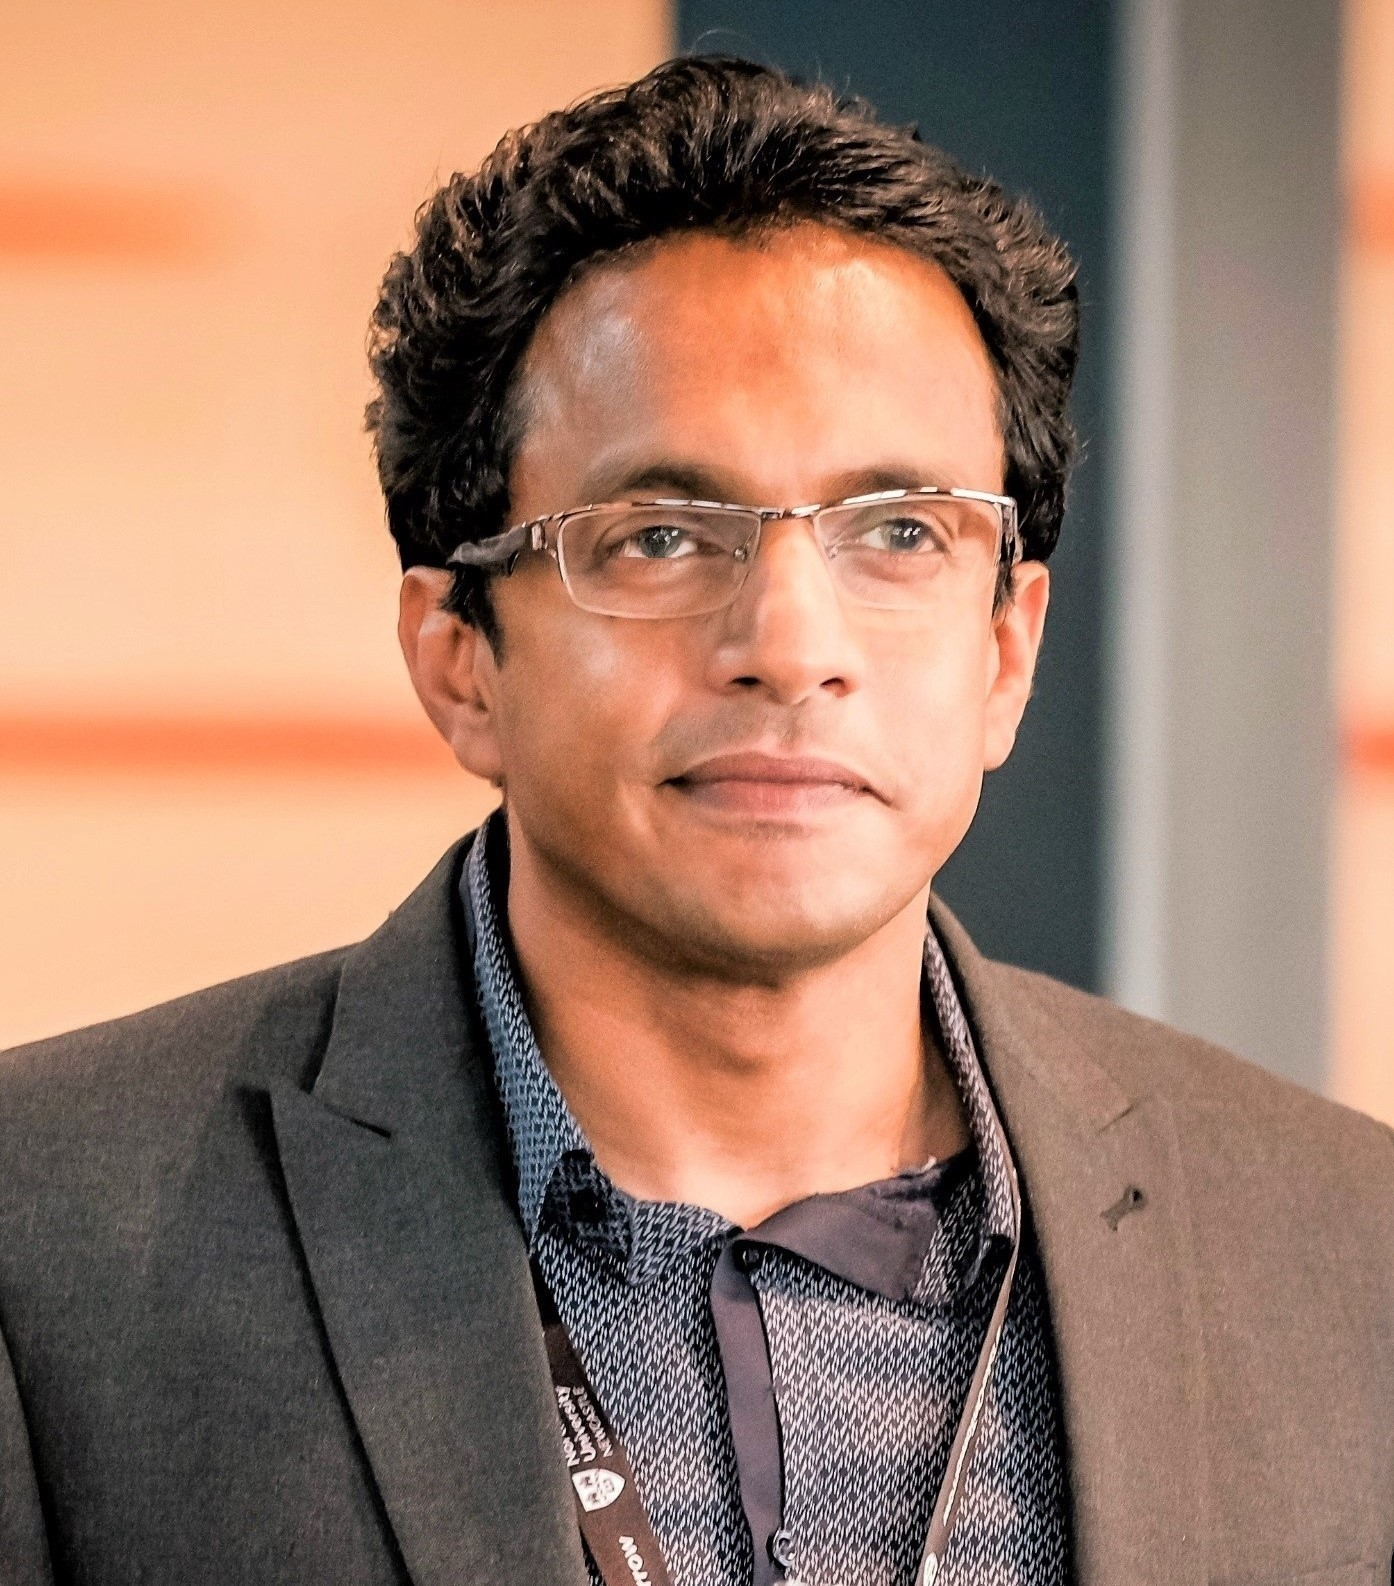
\includegraphics[width=1in,height=1.25in,clip,
keepaspectratio]{Figures/Biju.jpg}}]{Biju Issac}
received the B.E.\ degree in Electronics and Communications Engineering,
the Master of Computer Applications (MCA) degree, and the Ph.D.\ degree
in Networking and Mobile Communications.
He is an Associate Professor at Northumbria University, Newcastle Upon
Tyne, UK, and a Member of the IEEE.
He is research active and has authored more than 100 refereed conference
papers, journal articles, and book chapters.
His research interests include networks, cybersecurity, applied machine
learning, and deep learning.
\end{IEEEbiography}

\begin{IEEEbiography}[{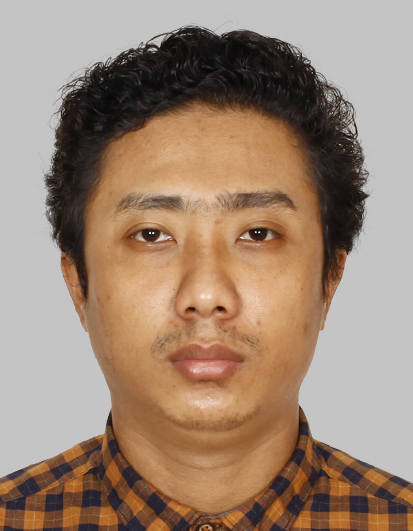
\includegraphics[width=1in,height=1.25in,clip,
keepaspectratio]{Figures/rahul.jpg}}]{Rahul Yumlembam}
completed his Ph.D.\ degree in Computer and Information Sciences at
Northumbria University, Newcastle Upon Tyne, UK.
He received the B.Tech.\ degree in Computer Science and Engineering and
the M.Tech.\ degree in Computer Science and Engineering (Artificial
Intelligence) in India, and was a Project Fellow at IIT Guwahati, India.
His research interests include machine learning, deep learning,
cybersecurity using AI, big data, brain--computer interface, text mining,
and image processing.
\end{IEEEbiography}

\begin{IEEEbiography}[{
\includegraphics[width=1in,height=1.25in,clip,
keepaspectratio]{Figures/Neera.JPG}}]{Jeyamohan Neera}
received the B.Sc.\ degree in Computer Engineering from the University
of Peradeniya, Sri Lanka, in 2008, and the M.Sc.\ degree in Information
Security from the University of Salford, UK, in 2012.
She completed her Ph.D.\ degree in Computer and Information Sciences at
Northumbria University, Newcastle Upon Tyne, UK.
She is currently an Assistant Professor and Programme Leader for Networks
and Cybersecurity, and serves as Expert Fellow for Security, Privacy,
Identity, and Trust in the Digital Economy (SPRITE+).
Her research interests include privacy in e-commerce systems, privacy
protection, privacy-enhanced AI, and cybersecurity.
\end{IEEEbiography}

\end{document}
